% Template for an EarthArXiv preprint of the manuscript.
% Includes the standard disclaimers and formatting that is required.
%
% This is the document structure. The actual content is written in:
% * abstract.tex: The abstract.
% * abstract-plain.tex: A plain language version of the abstract.
% * information.tex: Title, authors, journal, DOIs, dates.
% * content.tex: The actual manuscript text (minus the abstract).

%%%%%%%%%%%%%%%%%%%%%%%%%%%%%%%%%%%%%%%%%%%%%%%%%%%%%%%%%%%%%%%%%%%%%%%%%%%%%%%
% Set a class and import packages
\documentclass[onecolumn,10pt]{article}

\usepackage[utf8]{inputenc}
\usepackage[TU]{fontenc}
\usepackage[english]{babel}
\usepackage{amsmath}
\usepackage{amssymb}
\usepackage{graphicx}
\usepackage{hyperref}
\usepackage{fancyhdr}
\usepackage{orcidlink}
\usepackage{geometry}
\usepackage{booktabs}
\usepackage{microtype}
\usepackage{siunitx}
% To customize the title page
\usepackage{titling}
% For adding multiple authors
\usepackage{authblk}
% improved urls with proper hyphenation
\usepackage{xurl}
% Tweak the look of captions
\usepackage{caption}
% To control the style of section titles
\usepackage{titlesec}
% Import natbib and doi packages
\usepackage[round,authoryear,sort]{natbib}
% show dois as links on references
\usepackage{doi}
% Remove extra space between references
\usepackage{natbibspacing}
% Use a different font
\usepackage[scaled=1.1]{notomath}
% Icons and fonts (requires using xelatex or luatex)
\usepackage{fontawesome5}
\usepackage{academicons}
% Control the font size
\usepackage{anyfontsize}
\usepackage{setspace}
% To get the number of pages in the document
\usepackage{lastpage}
\usepackage{lipsum}
\usepackage{ragged2e}
\usepackage{mdframed}
% To define custom environments
\usepackage{environ}

%%%%%%%%%%%%%%%%%%%%%%%%%%%%%%%%%%%%%%%%%%%%%%%%%%%%%%%%%%%%%%%%%%%%%%%%%%%%%%%
% Import the title, authors, etc.
%%%%%%%%%%%%%%%%%%%%%%%%%%%%%%%%%%%%%%%%%%%%%%%%%%%%%%%%%%%%%%%%%%%%%%%%%%%%%%%
% Define information that is used to build the different documents, like the
% title, authors, affiliations, etc.

\newcommand{\Title}{Full vector inversion of magnetic microscopy images using Euler deconvolution as prior information}
\newcommand{\TitleShort}{Magnetic microscopy inversion}

\newcommand{\Year}{2024}
\newcommand{\SubmittedOn}{2023/06/01}
\newcommand{\AcceptedOn}{2024/04/11}

\newcommand{\GitHubRepository}{compgeolab/micromag-euler-dipole}
\newcommand{\ArchiveRepository}{10.6084/m9.figshare.22672978}

\newcommand{\PreprintDOI}{10.31223/X5QD5Z}
\newcommand{\Journal}{Geochemistry, Geophysics, Geosystems}
\newcommand{\JournalDOI}{10.1029/2023GC011082}

\newcommand{\Keywords}{%
  magnetic microscopy, geophysics, python, inverse problems, image processing
}

% NOTE: Author information is stored in the separate .tex files because the
% format varies between regular latex and journal formats...


%%%%%%%%%%%%%%%%%%%%%%%%%%%%%%%%%%%%%%%%%%%%%%%%%%%%%%%%%%%%%%%%%%%%%%%%%%%%%%%
% Configuration of the document

\geometry{%
  left=25mm,
  right=25mm,
  top=18mm,
  bottom=15mm,
  headsep=0mm,
  headheight=0mm,
  footskip=7mm,
  includehead=true,
  includefoot=true
}

% Control line and table row spacing
\onehalfspacing
\renewcommand{\arraystretch}{1.5}

% Set the spacing between bibliography entries (requires natbib)
\setlength{\bibsep}{0pt}

% Custom colors
\definecolor{darkgray}{gray}{0.4}
\definecolor{mediumgray}{gray}{0.5}
\definecolor{lightgray}{gray}{0.9}
\definecolor{mediumblue}{HTML}{2060c2}
\definecolor{lightblue}{HTML}{f7faff}

% Customize the title and author section
\setlength{\droptitle}{-2cm}
\pretitle{\begin{FlushLeft}\LARGE\bfseries}
\posttitle{\par\end{FlushLeft}{\color{lightgray}\hrule height 1.5pt}}
\preauthor{\begin{FlushLeft}\normalsize}
\postauthor{\par\end{FlushLeft}}
\predate{\begin{FlushLeft}\footnotesize}
\postdate{\par\end{FlushLeft}}

% Configure captions
\captionsetup[table]{position=below,skip=0pt}
\captionsetup{labelfont=bf,font={small,color=darkgray},skip=10pt}

% Make urls use the same font as every other text
\urlstyle{same}

% Configure hyperref and add PDF metadata
\hypersetup{
    colorlinks,
    allcolors=mediumblue,
    pdftitle={\Title},
    pdfauthor={\AuthorShort},
    breaklinks=true,
}

% Configure header and footer
% Inspired by LaPreprint: https://github.com/roaldarbol/LaPreprint
\newcommand{\Separator}{\hspace{3pt}|\hspace{3pt}}
\newcommand{\FooterFont}{\footnotesize\color{mediumgray}}
\pagestyle{fancy}
\fancyhf{}
\lfoot{%
  \FooterFont{}
  \AuthorShort{} (\Year)
  \Separator{}
  \TitleShort
}
\rfoot{%
  \FooterFont{}
  EarthArXiv
  \Separator{}
  \thepage\space of\space \pageref*{LastPage}
}
\renewcommand{\headrulewidth}{0pt}
\renewcommand{\footrulewidth}{1pt}
\preto{\footrule}{\color{lightgray}}
\fancypagestyle{plain}{%
  \fancyhf{}
  \lfoot{%
    \FooterFont{}
    \faCreativeCommons\faCreativeCommonsBy
    \Separator{}
    \textcopyright{} \Year{} The Authors
  }
  \rfoot{%
    \FooterFont{}
    doi:\href{https://doi.org/\PreprintDOI}{\PreprintDOI}
    \Separator{}
    EarthArXiv
    \Separator{}
    \thepage\space of\space \pageref*{LastPage}
  }
}

% Define fancy text boxes
\NewEnviron{summarybox}{%
  \mdfdefinestyle{summarybox_}{%
    leftline=true,
    rightline=false,
    topline=false,
    bottomline=false,
    linewidth=2pt,
    linecolor=mediumblue,
    backgroundcolor=lightblue,
    innertopmargin=12pt,
    innerbottommargin=12pt,
    innerleftmargin=12pt,
    innerrightmargin=12pt,
    skipbelow=10pt,
    skipabove=15pt,
  }
  \newmdenv[style=summarybox_]{summarybox_}
  \begin{summarybox_}
    \footnotesize
    \BODY
  \end{summarybox_}
}

%%%%%%%%%%%%%%%%%%%%%%%%%%%%%%%%%%%%%%%%%%%%%%%%%%%%%%%%%%%%%%%%%%%%%%%%%%%%%%%
\begin{document}

\maketitle
\vspace{-1cm}

\begin{summarybox}
  \noindent
  \textbf{Disclaimer:}
  This is a non-peer reviewed preprint of an article submitted for publication
  in \textit{\Journal{}}. It is available from EarthArXiv at
  \url{https://doi.org/\PreprintDOI}.
  %This is a peer-reviewed author-produced postprint of the article
  %``\AuthorShort{} (\Year). \Title. \textit{\Journal}.
  %doi:\href{https://doi.org/\JournalDOI}{\JournalDOI}''.
  %The postprint is available from EarthArXiv at
  %\url{https://doi.org/\PreprintDOI}.
  \\[0.25cm]
  \noindent
  \textbf{Open Science:}
  The source code used to generate all of the results presented in this
  research can be freely accessed and reused under the terms of an open license.
  You can find it at \url{https://doi.org/\ArchiveRepository} and
  \url{https://github.com/\GitHubRepository}.
  \\[0.25cm]
  \noindent
  \textbf{Keywords:} \Keywords{}
  \\[0.25cm]
  \noindent
  \textbf{\textcopyright{} \Year{} The Authors.}
  Available under the \href{https://creativecommons.org/licenses/by/4.0/}{Creative Commons Attribution 4.0 International License}
  \faCreativeCommons\faCreativeCommonsBy{}.
\end{summarybox}

\section*{\normalsize Abstract}
{\small Paleomagnetic data is collected from bulk samples, containing a mixture of stable and unstable magnetic particles. 
Recently, magnetic microscopy techniques have allowed the examination of individual magnetic grains. 
However, accurately determining the magnetic moments of these grains is difficult and time-consuming due to the inherent ambiguity of potential field data and the large number of grains in each image. 
Here we introduce a fast and semi-automated algorithm that estimates the position and magnetization of each magnetic source solely based on magnetic microscopy data, without requiring any additional information. 
The algorithm follows a three-step process. 
Firstly, it employs image processing techniques to identify and isolate data window boundaries for each magnetic source. 
Secondly, the algorithm uses Euler deconvolution to estimate their positioning. 
Lastly, the algorithm solves an overdetermined linear inverse problem, using a dipolar approximation, to determine the direction and intensity of the magnetic dipole moment for each source. 
To validate the algorithm, we conducted tests analyzing particle depth, intensity, and non-dipolarity. 
Additionally, synthetic data experiments were performed to demonstrate the effectiveness of the methodology in recovering the position and magnetic information of both dipolar and non-dipolar sources. 
These experiments included complex samples designed to simulate real rock data. 
While our underlying assumption is that of dipolar and spatially separated magnetic grains, our results show that the method is capable of automatically identifying individual dipolar sources that are at least between 14 and \qty{20}{\mu\meter} apart and can accurately recover the dipole moment and position of non-dipolar sources that are at least \qty{5}{\mu\meter} from the sensor.
However, the applicability of the method is still limited to particles in the single- or pseudosingle-domain range.
When applied to real data, our method is able to accurately retrieved the expected directions induced in the sample. 
The semi-automated nature of our algorithm, combined with its low processing cost and ability to simultaneously analyze the magnetic moments of numerous particles, represents a significant advancement in facilitating paleomagnetic applications of magnetic microscopy.}

\section*{\normalsize Plain language summary}
{\small Very small magnetic particles in rocks and other materials can store information about what the Earth’s magnetic field was like in the past. 
But not all particles are good recorders of this magnetic information, and some may have recorded different overlapping directions and strengths. 
So it is important to measure each particle separately in order to identify and separate the good recorders from the bad ones. 
A device called a ``quantum diamond microscope'' is able to measure the magnetic field near the surface of a rock sample at microscopic scale. 
We propose a new method for processing data from this microscope that is able to find out the individual magnetizations of large amounts small magnetic particles automatically.
We created a computer program to execute the method, which calculates the 3D position and magnetization of each particle using the simple model of a magnetic dipole. 
We tested the method on simulated data, using fake magnetic particles for which we know the correct magnetization and position, and real data, both of which showed good results in most cases. 
The method we created has the potential to enable the widespread study of the magnetism of natural materials with more detail than before.}

\section{Introduction}

Several branches of Earth Sciences have demonstrated the importance of the
``spatiality" of the data on a microscopic scale, mainly in geochemistry and
geochronology applications where it is possible to perform punctual analysis
and compositional maps, allowing significant advances in the understanding of
igneous, metamorphic and sedimentary processes \citep{Verberne2020, Barnes2019,
Davidson2007}. Classical paleomagnetic techniques, on the other hand, consist
in analyzing bulk samples, where the magnetic signal of a single specimen is
the result of the sum of moments of a large assembly of ferromagnetic grains
\citep{Dunlop1997}. Typically, a standard paleomagnetic sample of
approximately \qty{10}{\cm\cubed} would contain hundreds of thousands
to millions of magnetic particles with sizes varying from magnetically stable
single-domain (SD) and vortex state grains (also called pseudo-single domain,
PSD) with sizes below \qty{1}{\um}, to large ($\gg \qty{1}{\um}$) grains with
multi-domain (MD) magnetic structures, which are less stable magnetic recorders
\citep{Berndt2016}. These large MD grains usually conceal the signal of the SD
and PSD grains, and techniques of step-wise thermal and magnetic treatments are
needed to unveil the more stable and reliable magnetic record
\citep{Tauxe2018}. Recently, magnetic microscopy techniques opened the
possibility of performing magnetic maps at the micro-scale and recovering the
magnetization of each grain, therefore enabling the separate analysis of stable
and unstable magnetic particles \citep{DeGroot2018, Lima2014, Weiss2007,
DeGroot2014}.

In order to apply magnetic microscopy to paleomagnetic studies, it is necessary
to recover from the magnetic images a large amount of individual magnetic
moments, corresponding to at least tens of thousands of stable fine-grained
grains ($< \qty{1}{\um}$), in order to provide statistical significance to the
remanence vector \citep[e.g., ][]{Berndt2016}. Nowadays, with the development of
magnetic microscopy techniques, this task is no longer limited by the
resolution of magnetic microscopes \citep{Fu2020, Weiss2007, DeGroot2018,
Glenn2017, Lima2014}, but essentially by the intrinsic problem presented by the
ambiguity in the inversion of potential field data \citep{Barbosa2011,
DeGroot2021, Oliveira2015Estimation}, and ultimately by the lack of a fast and
automated way to recover such a large number of individual magnetic moments
from a set of magnetic images \citep{CortesOrtuno2022, Lima2013, Lima2009}. A
solution to the non-uniqueness of magnetic moment inversion is to add
independent prior information, such as the position of the ferromagnetic
particles \citep{Fabian2019}. This can be obtained, for example, from X-ray
computed tomography \citep[microCT; ][]{Fabian2019, DeGroot2021, DeGroot2018}.
Nonetheless, the standard microCT techniques do not provide adequate resolution
to resolve the finer and more stable magnetic grains \citep{CortesOrtuno2022,
DeGroot2021}, whereas other more sophisticated techniques such as ptychographic
X-ray tomography \citep[e.g., ][]{Maldanis2020} are not readily available and
too time-consuming to be routinely used in paleomagnetic studies.

Another route to be explored in the inversion of magnetic microscopy images is
to obtain all the information, i.e. the magnetic moment and the position of the
sources, from the magnetic data itself \citep[e.g., ][]{Fu2020}. For that, we can
explore the techniques developed in exploration geophysics, in spite of the
differences between aeromagnetic surveys and magnetic microscopy
\citep{Lima2013}. Magnetic microscopy images commonly show the combined signal
of multiple magnetic particles and can vary greatly in wavelength, strength,
and spatial separation, depending on the NRM and location of each particle. We
usually assume that the signal measured by the magnetic microscope is the
vertical component of the magnetic induction vector ($b_z$), the measurements
are performed on a regular grid with evenly spaced grid points and at a
constant height, and the data are contaminated with random Gaussian noise and
long-wavelength noise (akin to a regional signal in aeromagnetic data). Here,
we provide a methodological routine to retrieve the individual magnetic moment
of ferromagnetic grains in magnetic microscopy images following the approach
devised by \citet{Oliveira2015Estimation} for the interpretation of
aeromagnetic anomalies. The method we propose allows one to quickly and
semi-automatically estimate the individual magnetic moment vector of the stable
magnetic carriers, making use of only the magnetic images themselves and an
assumption of approximately dipolar sources. If used on a large scale, the
method provides the means to scan large areas of the rock sample, attaining
potentially the number of magnetic moments necessary for paleomagnetic studies.


%%%%%%%%%%%%%%%%%%%%%%%%%%%%%%%%%%%%%%%%%%%%%%%%%%%%%%%%%%%%%%%%%%%%%%%%%%%%%%%
\section{Methodology}

We will achieve the goal of estimating the dipole moment of several individual
grains per image in a semi-automatic fashion by dividing the task into three
parts that can be performed independently:

\begin{enumerate}
\item \textbf{Source detection and separation:} Identify and spatially isolate
  the magnetic field caused by each source. We will do this through a
  combination of classic potential field data processing (\textit{total
  gradient amplitude}) and image processing (histogram stretching and
  equalization) and segmentation methods (watershed segmentation).
\item \textbf{Position estimation}: Estimate the 3D position of a magnetic
  particle based on the magnetic field measurements and the assumption of a
  dipolar source. This can be achieved by applying the Euler Deconvolution
  method to the data segment identified in step 1.
\item \textbf{Magnetic moment inversion:} Estimate the 3-component dipole
  moment vector by inverting the magnetic field data using the position
  obtained from Euler Deconvolution as a constraint and the assumption of a
  dipolar source. This leads to a linear inverse problem that is stable and
  computationally efficient, particularly since the inversion is performed
  separately for each data segment identified in step 1.
\end{enumerate}

In the sections below, we describe the methodology used in each step of our
proposed workflow.

\subsection{Automatic source detection and separation}

Our first task is to automatically identify the signal of individual particles
and spatially segregate the data into windows, each containing the signal of a
single particle. We implemented the following workflow to achieve this:

\begin{enumerate}
\item Calculate the \textit{total gradient amplitude} (TGA), also known as the
  3D analytic signal \citep{Roest1992Magnetic}, of the observed vertical
  component of the magnetic field. The TGA is entirely positive and tends to be
  more concentrated on top of the magnetic field sources than the observed
  magnetic field. The derivative calculation also acts as a high-pass filter,
  removing long-wavelength noise from the data.
\item Apply a contrast stretching method to re-scale the TGA to a new range
  defined by the lower and upper percentiles of the data in order to highlight
  the weaker signals, either coming from small or from deep-seated particles.
\item Use the Laplacian of Gaussian (LoG) method \citep{Kong2013} on the
  re-scaled TGA data to estimate the position and size of data windows
  containing the signal of each particle.
\end{enumerate}

The total gradient amplitude (TGA) was devised as a filter that can be applied
to aeromagnetic data to reduce the signal's dependence on the direction of
magnetization of the source and that concentrates the signal above the sources
\citep{Roest1992Magnetic, Nabighian2005}. The TGA is defined as the norm of the
gradient vector of a scalar field $f(x, y, z)$

\begin{equation}
\|\vec{\mathbf{\nabla}}f(x, y, z)\|  = 
\sqrt{(\partial_x f)^2 + (\partial_y f)^2 + (\partial_z f)^2}
\ ,
\end{equation}

\noindent
in which $\partial_x f$ is the partial derivative of $f$ with respect to $x$
and likewise for the $y$ and $z$ directions. The partial derivatives are best
approximated using a second-order accurate central finite-difference scheme

\begin{equation}
\partial_x f(x, y, z) \approx 
\dfrac{f(x + \Delta x, y, z) - f(x - \Delta x, y, z)}{2 \Delta x} 
\ ,
\end{equation}

\noindent
and likewise for the $y$ and $z$ directions, in which $\Delta x$ is the grid
spacing (assumed to be equal in the $x$ and $y$ directions). For the $z$
component, $\Delta z = \Delta x$ and $f(x, y, z + \Delta z)$ and
$f(x, y, z - \Delta z)$ are calculated by upward and downward continuation,
respectively, performed in the wavenumber domain. The 2D maps of the $x$, $y$,
and $z$ derivatives will also be used in the Euler Deconvolution step described
below, which is known to be highly sensitive to noise in the derivatives
\citep{Saleh2012Applying}. This is why e prefer the finite-differences based
derivatives, which are less prone to amplifying short-wavelength noise than
those calculated in the wavenumber domain through the Fast Fourier Transform
(FFT).

Once we have obtained a TGA image, we apply a contrast stretching method to
re-scale the TGA values in order to highlight the weaker signals present in the
image. This is a necessary step to make sure that the blob detection algorithm
is able to identify particles causing both weak and strong signals. The
following contrast stretching operation is performed per pixel of the TGA image

\begin{equation}
\text{TGA}_{rescaled} = 
2\left(\dfrac{\text{TGA} - v_{min}}{v_{max} - v_{min}}\right) - 1 
\ ,
\end{equation}

\noindent
in which $v_{min}$ and $v_{max}$ are the upper and lower bounds of TGA values
that will be stretched to the range $[0, 1]$. By experimentation, we found
that values of $v_{min} = 1^\text{st}$ and $v_{max} = 99^\text{th}$
percentiles of the TGA range work well on real magnetic microscopy datasets.

The re-scaled TGA image is then used as input for a Laplacian of Gaussian (LoG)
blob detection algorithm \citep{Kong2013}. This method is able to identify the
location and size of multiple windows in the image containing ``blobs''. In our
case, the blobs are the re-scaled TGA field of each particle and the LoG method
detects the local TGA maxima. The LoG method is particularly well suited for
the detection of bright blobs on a dark background at the expense of a longer
computation time \citep{Han2016}. For the image sizes routinely found in
magnetic microscopy, the computation is fast and only needs to be performed
once per image.

\subsection{Euler Deconvolution}

Once the locations and sizes of the windows containing the isolated signals of
each particle are determined, we can apply the Euler Deconvolution (ED)
estimate of the $x$, $y$, and $z$ positions of the center of the particles
under a dipolar approximation. This technique was first proposed by
\citet{Thompson1982} under the name EULDPH and later extended to three
dimensions and renamed ``Euler Deconvolution'' by \citet{Reid1990}. ED is
traditionally performed on a set of moving windows that scan the entire
dataset, producing a large scatter of position estimates, most of which are
spurious \citep{Silva20033D}. This is only done because it is impractical to
segment an aeromagnetic dataset into individual anomalies. Fortunately,
magnetic microscopy images contain fewer elongated features (e.g., dikes and
suture zones) and regional signals (e.g., Curie depth variations) that are
difficult to separate. This makes it possible for us to produce isolated
signals for each magnetic particle through the source detection step described
above. Since each data window contains only the signal of a single particle, we
are able to apply ED and generate only a single position estimate per particle.

\begin{figure}[t]
\centering
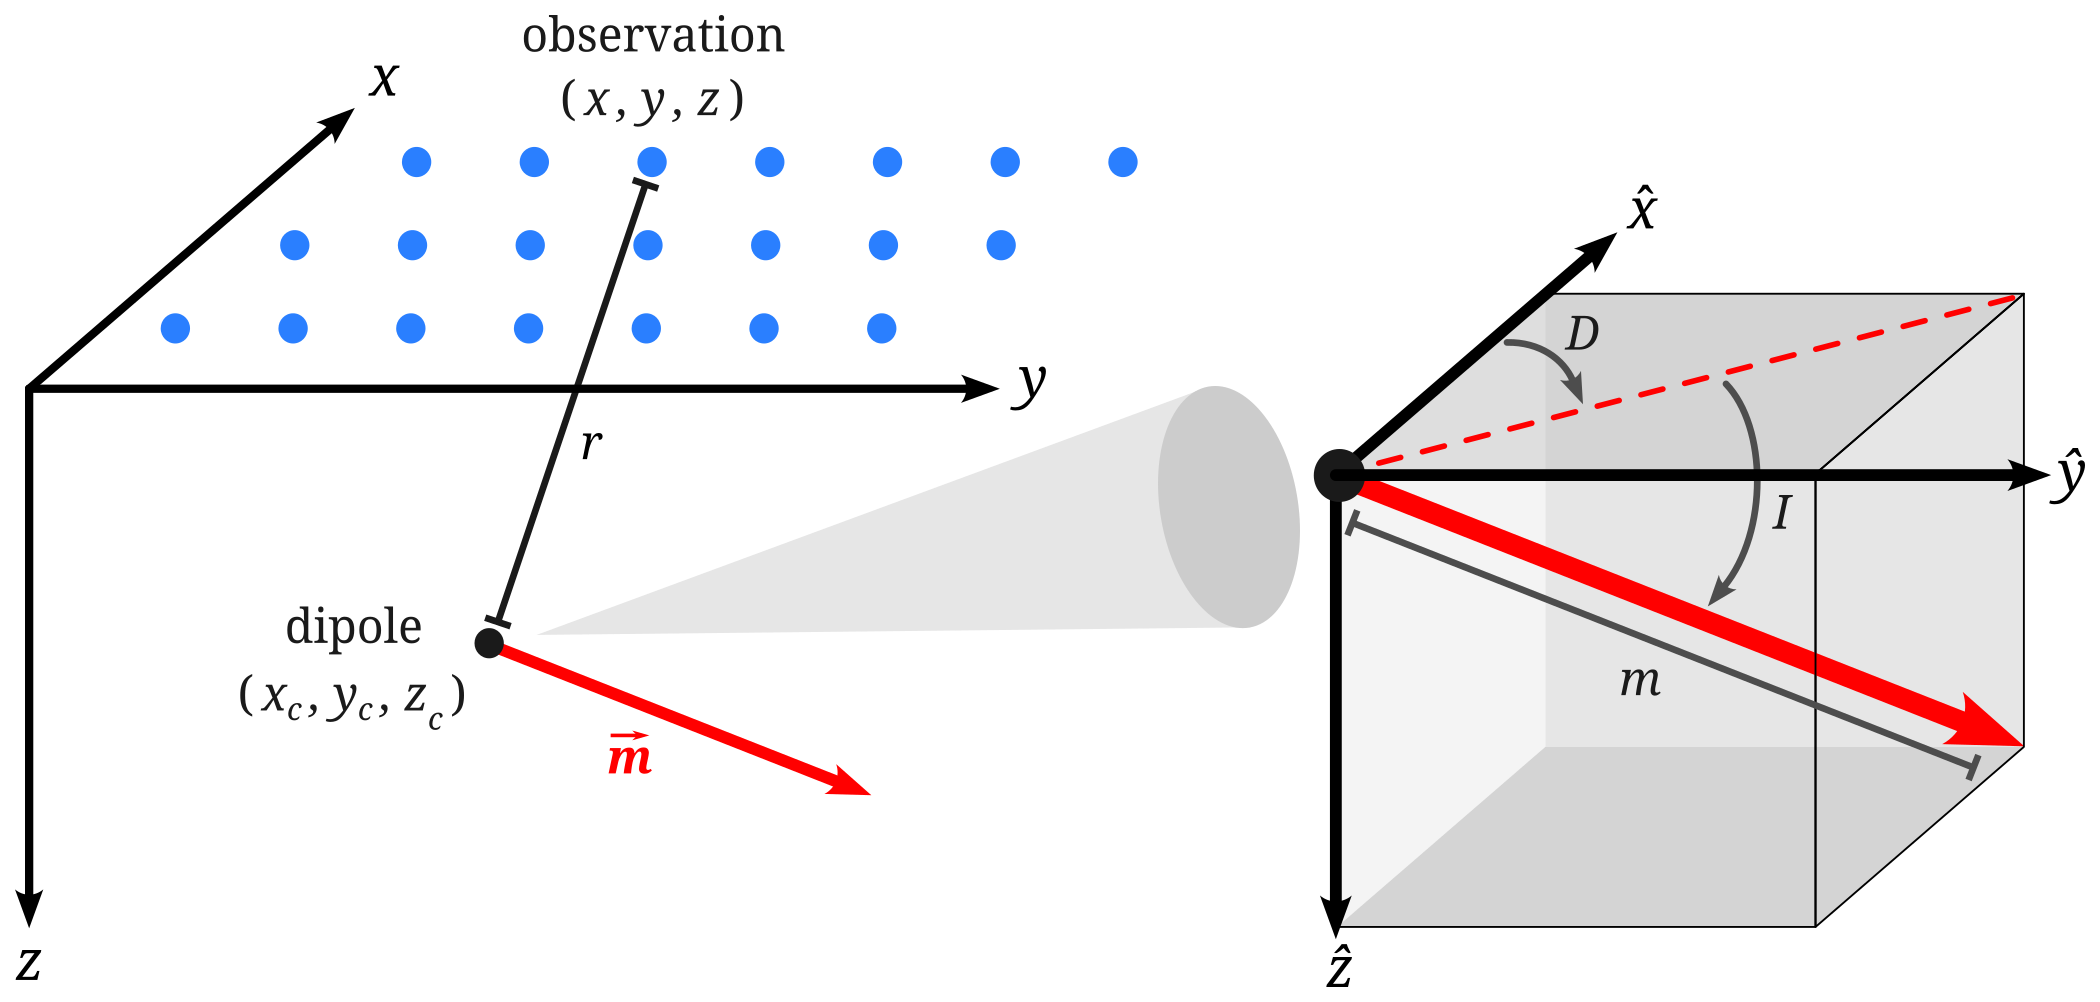
\includegraphics[width=\linewidth]{figures/coordinate-system-sketch.png}
\caption{
Schematic representation of the coordinates systems and modelling elements.
The left panel shows the $x, y, z$ right-handed coordinate system with $z$ 
pointing upward and away from the sample. A dipole with dipole moment vector 
$\mathbf{\vec{m}}$ is also shown at coordinates $(x_c, y_c, z_c)$. The 
observation points are located at regular intervals on an $x-y$ plane. 
The right panel zooms in on the dipole and shows the dipole moment vector
expressed in terms of inclination ($I$, positive downwards), declination
($D$, angle with the $\hat{y}$ direction), and moment magnitude
$m = \|\mathbf{m}\|$.
}
\label{fig_coordinate_systems}
\end{figure}

Euler Deconvolution is formulated as a least-squares inversion of Euler's
homogeneity equation

\begin{equation}
\label{eq_euler_homogeneity}
(x - x_c)\partial_x f
+ (y - y_c)\partial_y f
+ (z - z_c)\partial_z f
= (b - f)\eta
\ ,
\end{equation}

\noindent
in which $(x_c, y_c, z_c)$ are the coordinates of the magnetic field source
(Figure~\ref{fig_coordinate_systems}), $b$ is the base level representing a
constant shift in the signal, and $\eta$ is the structural index corresponding
to the nature of the source \citep{Reid1990}. This equation holds true for
simple geometric sources, like spheres, dipoles, and vertical cylinders. Here,
we assume that the magnetic particles are small enough and the sensor is far
enough away that the sources can be represented by dipoles, yielding an
$\eta=3$.

The inversion is performed by rearranging Equation~\ref{eq_euler_homogeneity}
into a pseudo-parametric model with parameters $x_c$, $y_c$, $z_c$, and $b$

\begin{equation}
x_c \partial_x f + y_c \partial_x f + z_c \partial_x f + \eta b
=
x \partial_x f + y \partial_y f + z \partial_z f + \eta f
\ .
\end{equation}

Given a set of $N$ observations of the magnetic field as the harmonic function
$f$ and its spatial derivatives, we can form the $N \times 4$ system of
equations

\begin{equation}
\begin{bmatrix}
  {\partial_x f}_1 & {\partial_y f}_1 & {\partial_z f}_1 & \eta \\
  {\partial_x f}_2 & {\partial_y f}_2 & {\partial_z f}_2 & \eta \\
  \vdots & \vdots & \vdots & \vdots \\
  {\partial_x f}_N & {\partial_y f}_N & {\partial_z f}_N & \eta
\end{bmatrix}
\begin{bmatrix}
  x_c \\ y_c \\ z_c \\ b
\end{bmatrix}
=
\begin{bmatrix}
  x_1 {\partial_x f}_1 + y_1 {\partial_y f}_1 + z_1 {\partial_z f}_1 + \eta f_1 \\
  x_2 {\partial_x f}_2 + y_2 {\partial_y f}_2 + z_2 {\partial_z f}_2 + \eta f_2 \\
  \vdots \\
  x_N {\partial_x f}_N + y_N {\partial_y f}_N + z_N {\partial_z f}_N + \eta f_N \\
\end{bmatrix}
\ .
\end{equation}

In matrix notation, this linear system can be written as

\begin{equation}
\label{eq_euler_forward}
\mathbf{G} \mathbf{p} = \mathbf{h} \ .
\end{equation}

We can arrive at a solution to Equation~\ref{eq_euler_forward} by assuming that
the three spatial derivatives of $f$ have negligible error and minimizing the
misfit $\phi(\mathbf{p})$ between a pseudo-observation vector $\mathbf{h}^o$
and the predictions $\mathbf{h}$. The least-squares misfit $\phi(\mathbf{p})$
is defined as

\begin{equation}
\label{ZTSuSBbL16}
\phi(\mathbf{p}) = \|\mathbf{h}^o - \mathbf{h}\|^2 = (\mathbf{h}^o - \mathbf{G}\mathbf{p})^T (\mathbf{h}^o - \mathbf{G}\mathbf{p})\ .
\end{equation}

The minimum of $\phi(\mathbf{p})$ is obtained by solving the $4 \times 4$
system of normal equations

\begin{equation}
\mathbf{G}^T \mathbf{G} \mathbf{p} = \mathbf{G}^T \mathbf{h}^o\ .
\end{equation}

The solution vector $\hat{\mathbf{p}}$ provides an estimate of the position
$(x_c, y_c, z_c)$ and base level $b$ for the source located inside of a data
window. Repeating this process for each window produced by the source detection
algorithm will yield the horizontal locations and depths of each magnetic
particle.

\subsection{Magnetic moment inversion}

Once the source position is known and we can assume that it is approximately
spherical or dipolar, we can apply the method developed by
\citet{Oliveira2015Estimation} to estimate the dipole moment vector
$\mathbf{m}$ of the source. We begin by following
\citet{Oliveira2015Estimation} in formulating the magnetic induction vector
$\mathbf{b}$ of a dipole as

\begin{equation}
\label{eq_vector_dipole_field}
\mathbf{b}
=
\begin{bmatrix}
  b_x \\ b_y \\ b_z
\end{bmatrix}
= \dfrac{\mu_0}{4\pi}
\begin{bmatrix}
    \dfrac{\partial^2}{\partial x \partial x} \dfrac{1}{r}
  & \dfrac{\partial^2}{\partial x \partial y} \dfrac{1}{r}
  & \dfrac{\partial^2}{\partial x \partial z} \dfrac{1}{r}
  \\
    \dfrac{\partial^2}{\partial y \partial x} \dfrac{1}{r}
  & \dfrac{\partial^2}{\partial y \partial y} \dfrac{1}{r}
  & \dfrac{\partial^2}{\partial y \partial z} \dfrac{1}{r}
  \\
  \dfrac{\partial^2}{\partial z \partial x} \dfrac{1}{r}
  & \dfrac{\partial^2}{\partial z \partial y} \dfrac{1}{r}
  & \dfrac{\partial^2}{\partial z \partial z} \dfrac{1}{r}
\end{bmatrix}
\begin{bmatrix}
  m_x \\ m_y \\ m_z
\end{bmatrix}
= \dfrac{\mu_0}{4\pi} \mathbf{M}\,\mathbf{m}
\ ,
\end{equation}

\noindent
in which $r = \sqrt{(x - x_c)^2 + (y - y_c)^2 + (z - z_c)^2}$ is the Cartesian
distance between the observation point $(x, y, z)$ and the source $(x_c, y_c,
z_c)$ and $\mu_0$ is the vacuum magnetic permeability. Most magnetic
microscopes provide measurements of only the vertical component $b_z$, which
can be isolated from Equation~\ref{eq_vector_dipole_field} as

\begin{equation}
\label{eq_dipole_bz}
b_z
= \dfrac{\mu_0}{4\pi}
\begin{bmatrix}
\dfrac{\partial^2}{\partial z \partial x} \dfrac{1}{r}
& \dfrac{\partial^2}{\partial z \partial y} \dfrac{1}{r}
& \dfrac{\partial^2}{\partial z \partial z} \dfrac{1}{r}
\end{bmatrix}
\begin{bmatrix}
m_x \\ m_y \\ m_z
\end{bmatrix}
= \dfrac{\mu_0}{4\pi} \mathbf{M_z}\,\mathbf{m}
\ .
\end{equation}

The three second-order derivatives in Equation~\ref{eq_dipole_bz} are

\begin{equation}
\begin{aligned}
\dfrac{\partial^2}{\partial z \partial x} \dfrac{1}{r} &=
\dfrac{3(z - z_c)(x - x_c)}{r^5}\ ,
\\
\dfrac{\partial^2}{\partial z \partial y} \dfrac{1}{r} &=
\dfrac{3(z - z_c)(y - y_c)}{r^5}\ ,
\\
\dfrac{\partial^2}{\partial z \partial z} \dfrac{1}{r} &=
\dfrac{3(z - z_c)^2}{r^5} - \dfrac{1}{r^3}\ .
\end{aligned}
\end{equation}

Given a set of $N$ observations of $b_z$ made inside a window containing a
single source, we can form the $N \times 3$ linear equation system

\begin{equation}
\label{CgjOtKLQKT}
\begin{bmatrix}
\dfrac{\mu_0}{4\pi}\dfrac{3(z_1 - z_c)(x_1 - x_c)}{r_1^5}
& \dfrac{\mu_0}{4\pi}\dfrac{3(z_1 - z_c)(y_1 - y_c)}{r_1^5}
& \dfrac{\mu_0}{4\pi}\left(\dfrac{3(z_1 - z_c)^2}{r_1^5} - \dfrac{1}{r_1^3}\right)
\\
\dfrac{\mu_0}{4\pi}\dfrac{3(z_2 - z_c)(x_2 - x_c)}{r_2^5}
& \dfrac{\mu_0}{4\pi}\dfrac{3(z_2 - z_c)(y_2 - y_c)}{r_2^5}
& \dfrac{\mu_0}{4\pi}\left(\dfrac{3(z_2 - z_c)^2}{r_2^5} - \dfrac{1}{r_2^3}\right)
\\
\vdots & \vdots & \vdots
\\
\dfrac{\mu_0}{4\pi}\dfrac{3(z_N - z_c)(x_N - x_c)}{r_N^5}
& \dfrac{\mu_0}{4\pi}\dfrac{3(z_N - z_c)(y_N - y_c)}{r_N^5}
& \dfrac{\mu_0}{4\pi}\left(\dfrac{3(z_N - z_c)^2}{r_N^5} - \dfrac{1}{r_N^3}\right)
\end{bmatrix}
\begin{bmatrix}
m_x \\ m_y \\ m_z
\end{bmatrix}
=
\begin{bmatrix}
{b_z}_1 \\ {b_z}_2 \\ \vdots \\ {b_z}_L
\end{bmatrix}
\ ,
\end{equation}

\noindent
which can also be expressed in matrix form as

\begin{equation}
\label{qdhqM4s9Ln}
\mathbf{A} \mathbf{m} = \mathbf{d} \ .
\end{equation}

As with Euler Deconvolution, we can find a dipole moment vector that best fits
a set of $N$ observations of the vertical component of the magnetic field
$\mathbf{d}^o$ in a least-squares sense by minimizing the misfit function

\begin{equation}
\label{uV9pRVYO4l}
\Gamma (\mathbf{m}) = \| \mathbf{d}^o - \mathbf{d} \|^2 = (\mathbf{d}^o - \mathbf{A}\mathbf{m})^T  (\mathbf{d}^o - \mathbf{A}\mathbf{m})\ .
\end{equation}

\noindent
The dipole moment vector that minimizes $\Gamma (\mathbf{m})$ can be found by
solving the $3 \times 3$ normal equation system

\begin{equation}
\mathbf{A}^T \mathbf{A} \mathbf{m} = \mathbf{A}^T\mathbf{d}^o\ .
\end{equation}

\noindent
The estimated dipole moment vector $\hat{\mathbf{m}}$ can be converted into
declination $D$, inclination $I$, and magnitude $m$, which are more intuitive
quantities for interpreting paleomagnetic results, like so

\begin{equation}
  \label{eq_vector_to_incdec}
\begin{aligned}
I &= \tan^{-1}\left(\dfrac{m_z}{\sqrt{m_x^2 + m_y^2}}\right) \ , \\
D &= \tan^{-1}\left(\dfrac{m_x}{m_y}\right) \ , \\
m &= \sqrt{m_x^2 + m_y^2 + m_z^2} \ .
\end{aligned}
\end{equation}

It's important to note that these are not paleomagnetic declination and
inclination angles, but are instead related to the sample coordinate system. To
obtain the paleomagnetic direction, the dipole moment vector must be rotated to
the sample field orientation prior to the application of
Equation~\ref{eq_vector_to_incdec}.

MISSING PARAGRAPH ABOUT THE COVARIANCE ESTIMATION AND $\sigma_0$.

\begin{equation}
\label{lPOQaqlV3N}
\mathbf{C} =
\begin{bmatrix}
\sigma_x^2 & \sigma_{xy} & \sigma_{xz} \\
\sigma_{yx} & \sigma_y^2 & \sigma_{yz} \\
\sigma_{zx} & \sigma_{zy} & \sigma_z^2
\end{bmatrix}
=
\sigma_0^2 (\mathbf{A}^T\mathbf{A})^{-1}
\end{equation}

From the main diagonal of $\mathbf{C}$ we can obtain the variances of the
declination $\sigma_D^2$, inclination $\sigma_I^2$, and magnitude $\sigma_m^2$
by propagation of uncertainties

\begin{equation}
\begin{aligned}
\sigma_D^2 &= \dfrac{m_y^2\sigma_x^2 + m_x^2\sigma_y^2}{\left(m_x^2 + m_y^2\right)^2} \ , \\
\sigma_I^2 &= \dfrac{m_x^2 m_z^2 \sigma_x^2 + m_y^2 m_z^2 \sigma_y^2 + \left(m_x^2 + m_y^2\right)^2\sigma_z^2}{\left(m_x^2 + m_y^2\right) m^4} \ , \\
\sigma_m^2 &= \dfrac{m_x^2\sigma_x^2 + m_y^2\sigma_y^2 + m_z^2\sigma_z^2}{m^2} \ .
\end{aligned}
\end{equation}

\noindent
These variances reflect the sensitivity of the estimated dipole moment to
random noise in the magnetic field observations. However, they do not capture
other, often larger, sources of uncertainty like systematic errors in the
observations, data positioning errors, and the validity of the dipolar
approximation. Therefore, we recommend that these estimated variances be
treated with caution and should not be interpreted as ``the degree of certainty
that the estimated values are the true values''.

[FALAR SOBRE O CALCULO DE R2]

[INCLUIR A ESTIMATIVA DE NÃO-DIPOLARIDADE]


%%%%%%%%%%%%%%%%%%%%%%%%%%%%%%%%%%%%%%%%%%%%%%%%%%%%%%%%%%%%%%%%%%%%%%%%%%%%%%%
\section{Application to synthetic data}

We first applied our inversion workflow to synthetic data to evaluate its
strengths and limitations. The first set of synthetic data is simple and
intended to test the method's performance under ideal circumstances. The second
set is more complex, with a greater number of magnetic particles and
long-wavelength noise, and is intended to demonstrate the capabilities and
limitations of the method under real-world scenarios.

The first synthetic model was performed by generating the vertical magnetic
field derived from a simple set of four spheres with similar magnetization
intensity and radius, but completely different magnetization directions,
contaminated by high-frequency noise. This simplified test model is basically
done to investigate the efficiency of the inversions used for Euler positioning
and magnetization parameters, thus being a validation of the methodology.

The second model contains one hundred spheres with different radii and
magnetization intensities but magnetized in a similar direction within one
standard deviation. The magnetic field generated from these sources is
corrupted by both low and high-frequency noise. The complexity of this
synthetic data seeks to more faithfully emulate real magnetic microscopy data.


\subsection{Simple simulation: Validating the methodology}

\begin{figure}[tbp]
\centering
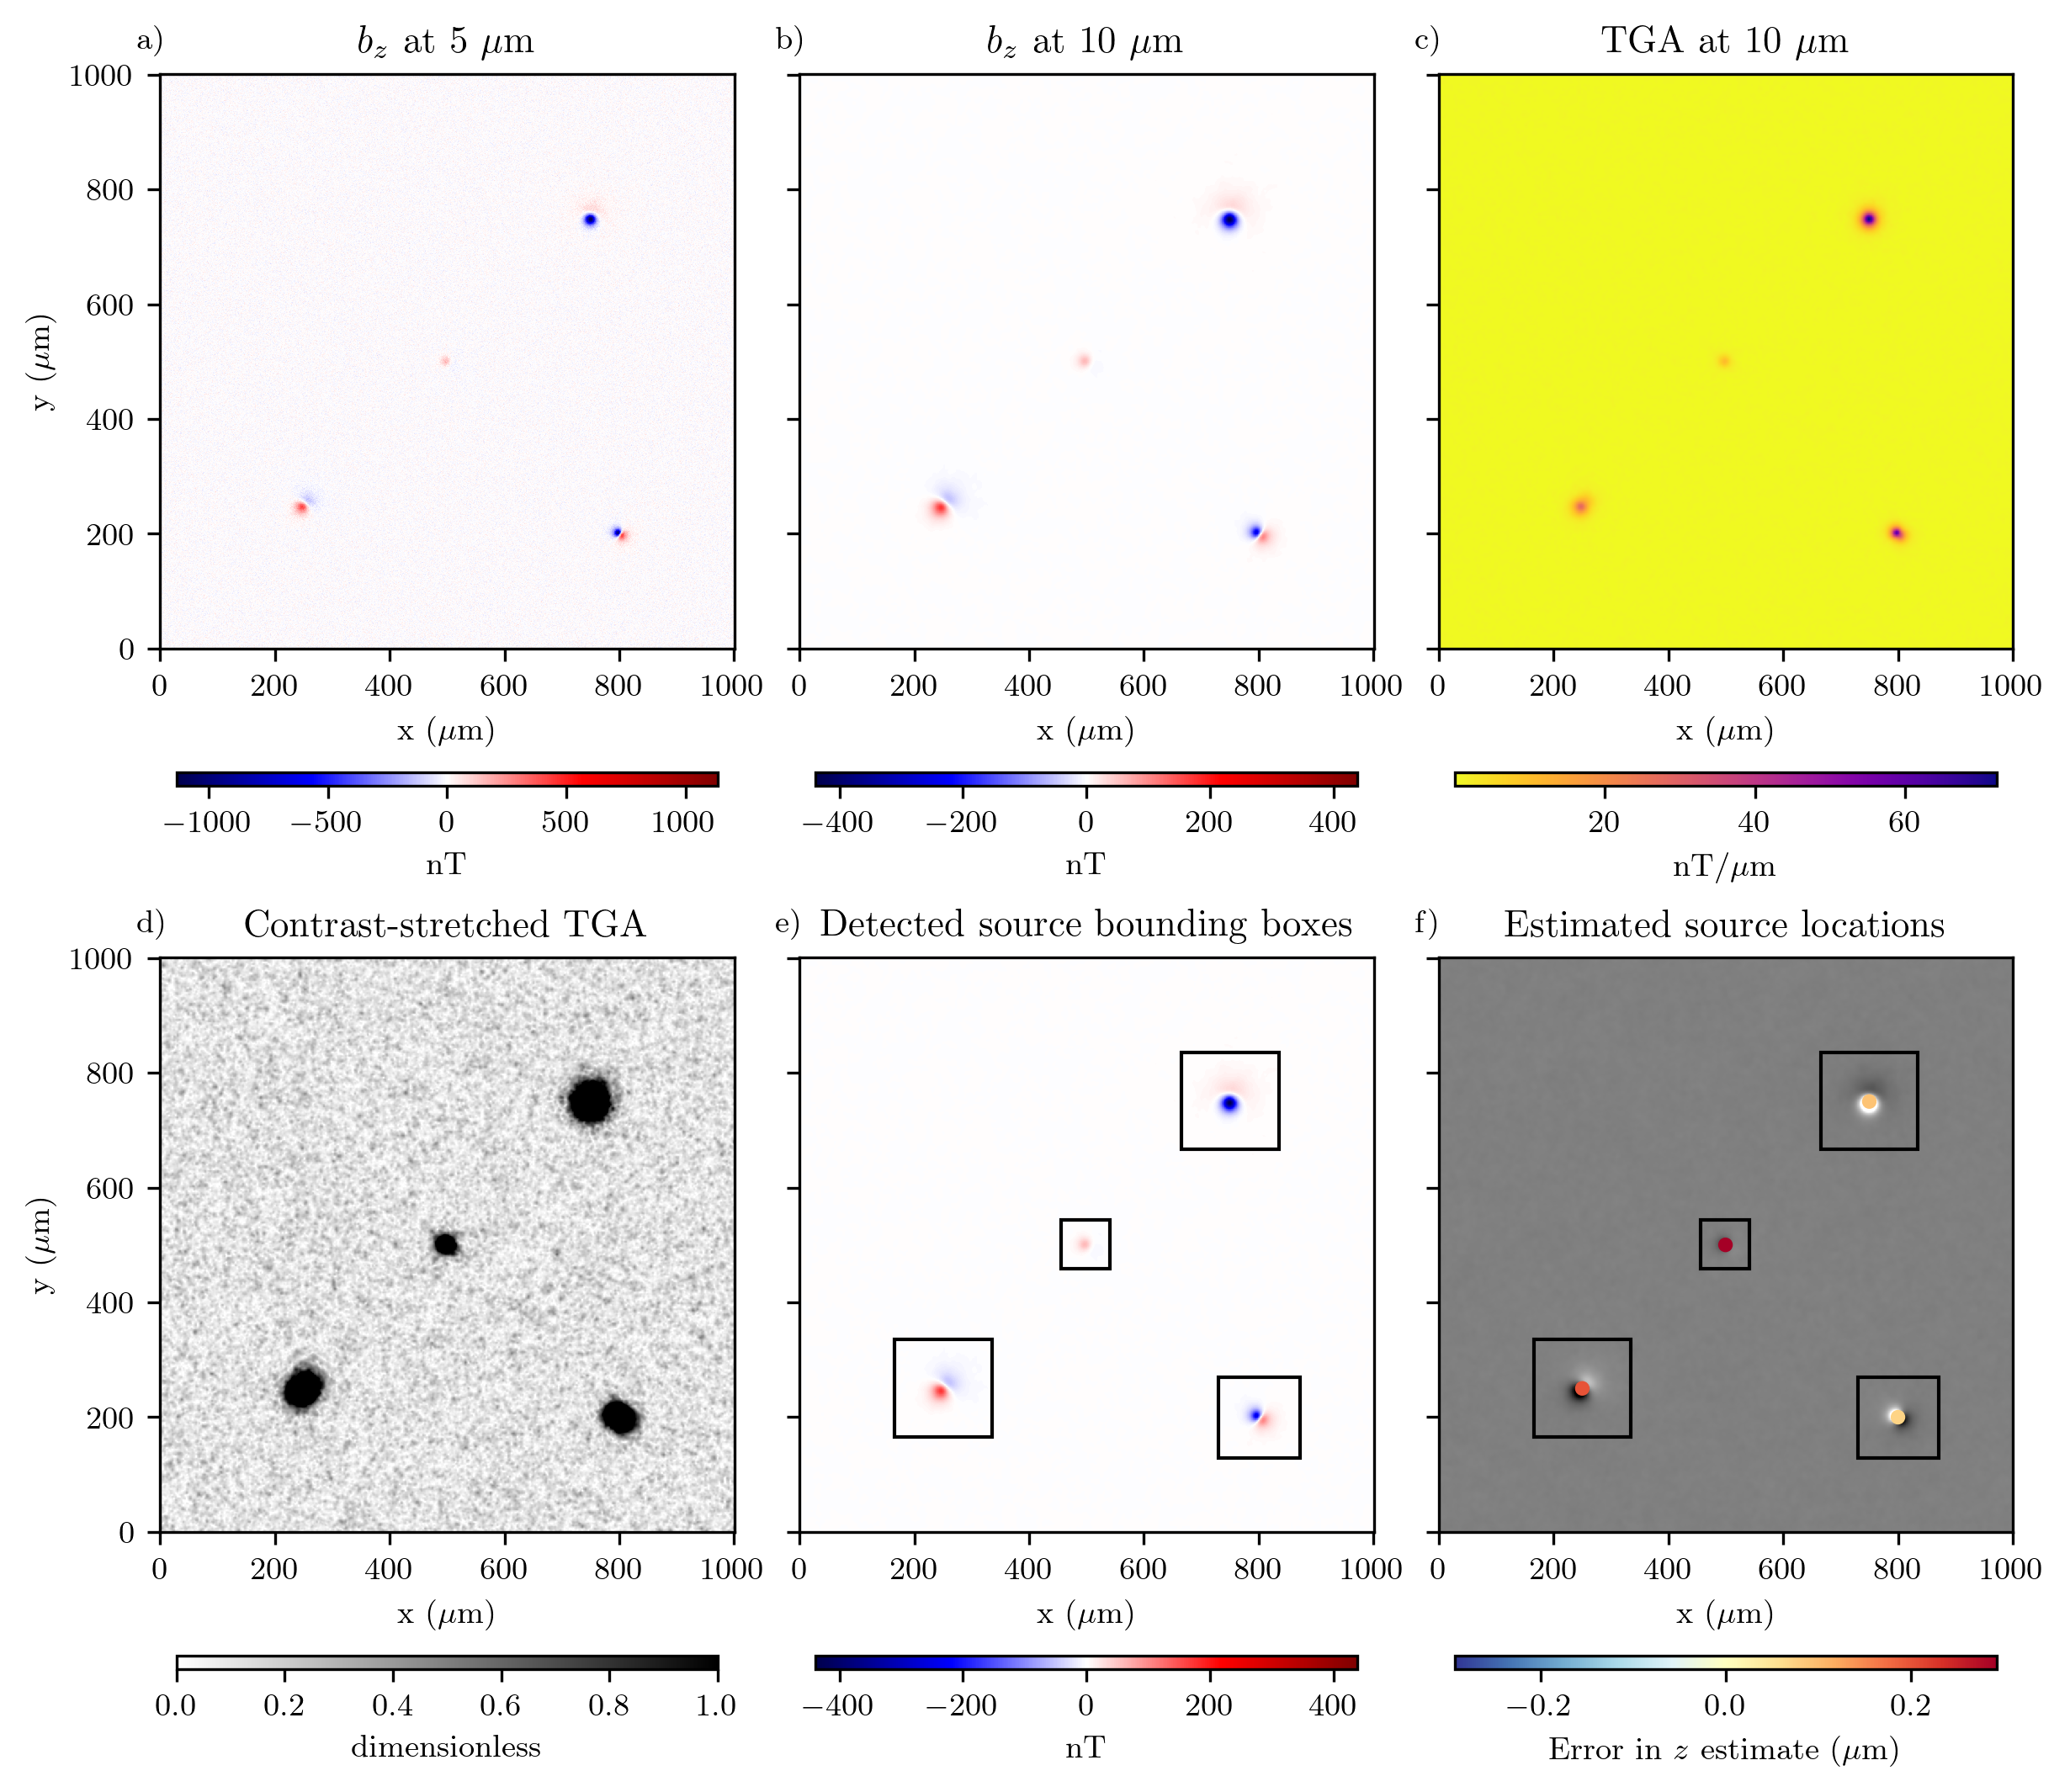
\includegraphics[width=1\linewidth]{figures/simple-synthetic-data.png}
\caption{
  a) Synthetic data contaminated with psedo-random normal noise. b) Individual sources window position (yellow squares) obtained with the blob detection algorithm applied on the total gradient map.
}
\label{fig_synthetic_simple_data}
\end{figure}

Figure~\ref{fig_synthetic_simple_data}a shows the vertical component of the magnetic field
$b_z$ over a synthetic rock section containing four uniformly magnetized
spherical sources. The map covers a surface of $\qty{1000}{\um} \times
\qty{1000}{\um}$ with
data points in a regular grid of \qty{1}{\um} ($N = 10^6$ observations)
obtained at a sensor-sample distance of \qty{5}{\um}. The magnetic field data is
contaminated with a pseudo-random noise of normal Gaussian distribution with a
zero mean and \qty{20}{\nano\tesla} standard deviation.

We first applied an upward continuation filter to smooth out high-frequency
noise \citep{Blakely1996}, since it strongly affects the first derivatives of
the potential field required by the Euler equation. Then, we calculated the
magnetic total gradient (or horizontal gradient) filter and applied the blob
detection algorithm to the total gradient map to obtain the position of the
data window for each source (Figure~\ref{fig_coordinate_systems}b). The ED was
run for each selected source by assuming the structural index of a
sphere/punctual source, therefore obtaining the Cartesian coordinates of each
source causing the magnetic potential anomaly in the observed data set (Table
1).

\begin{figure}[!t]
\centering
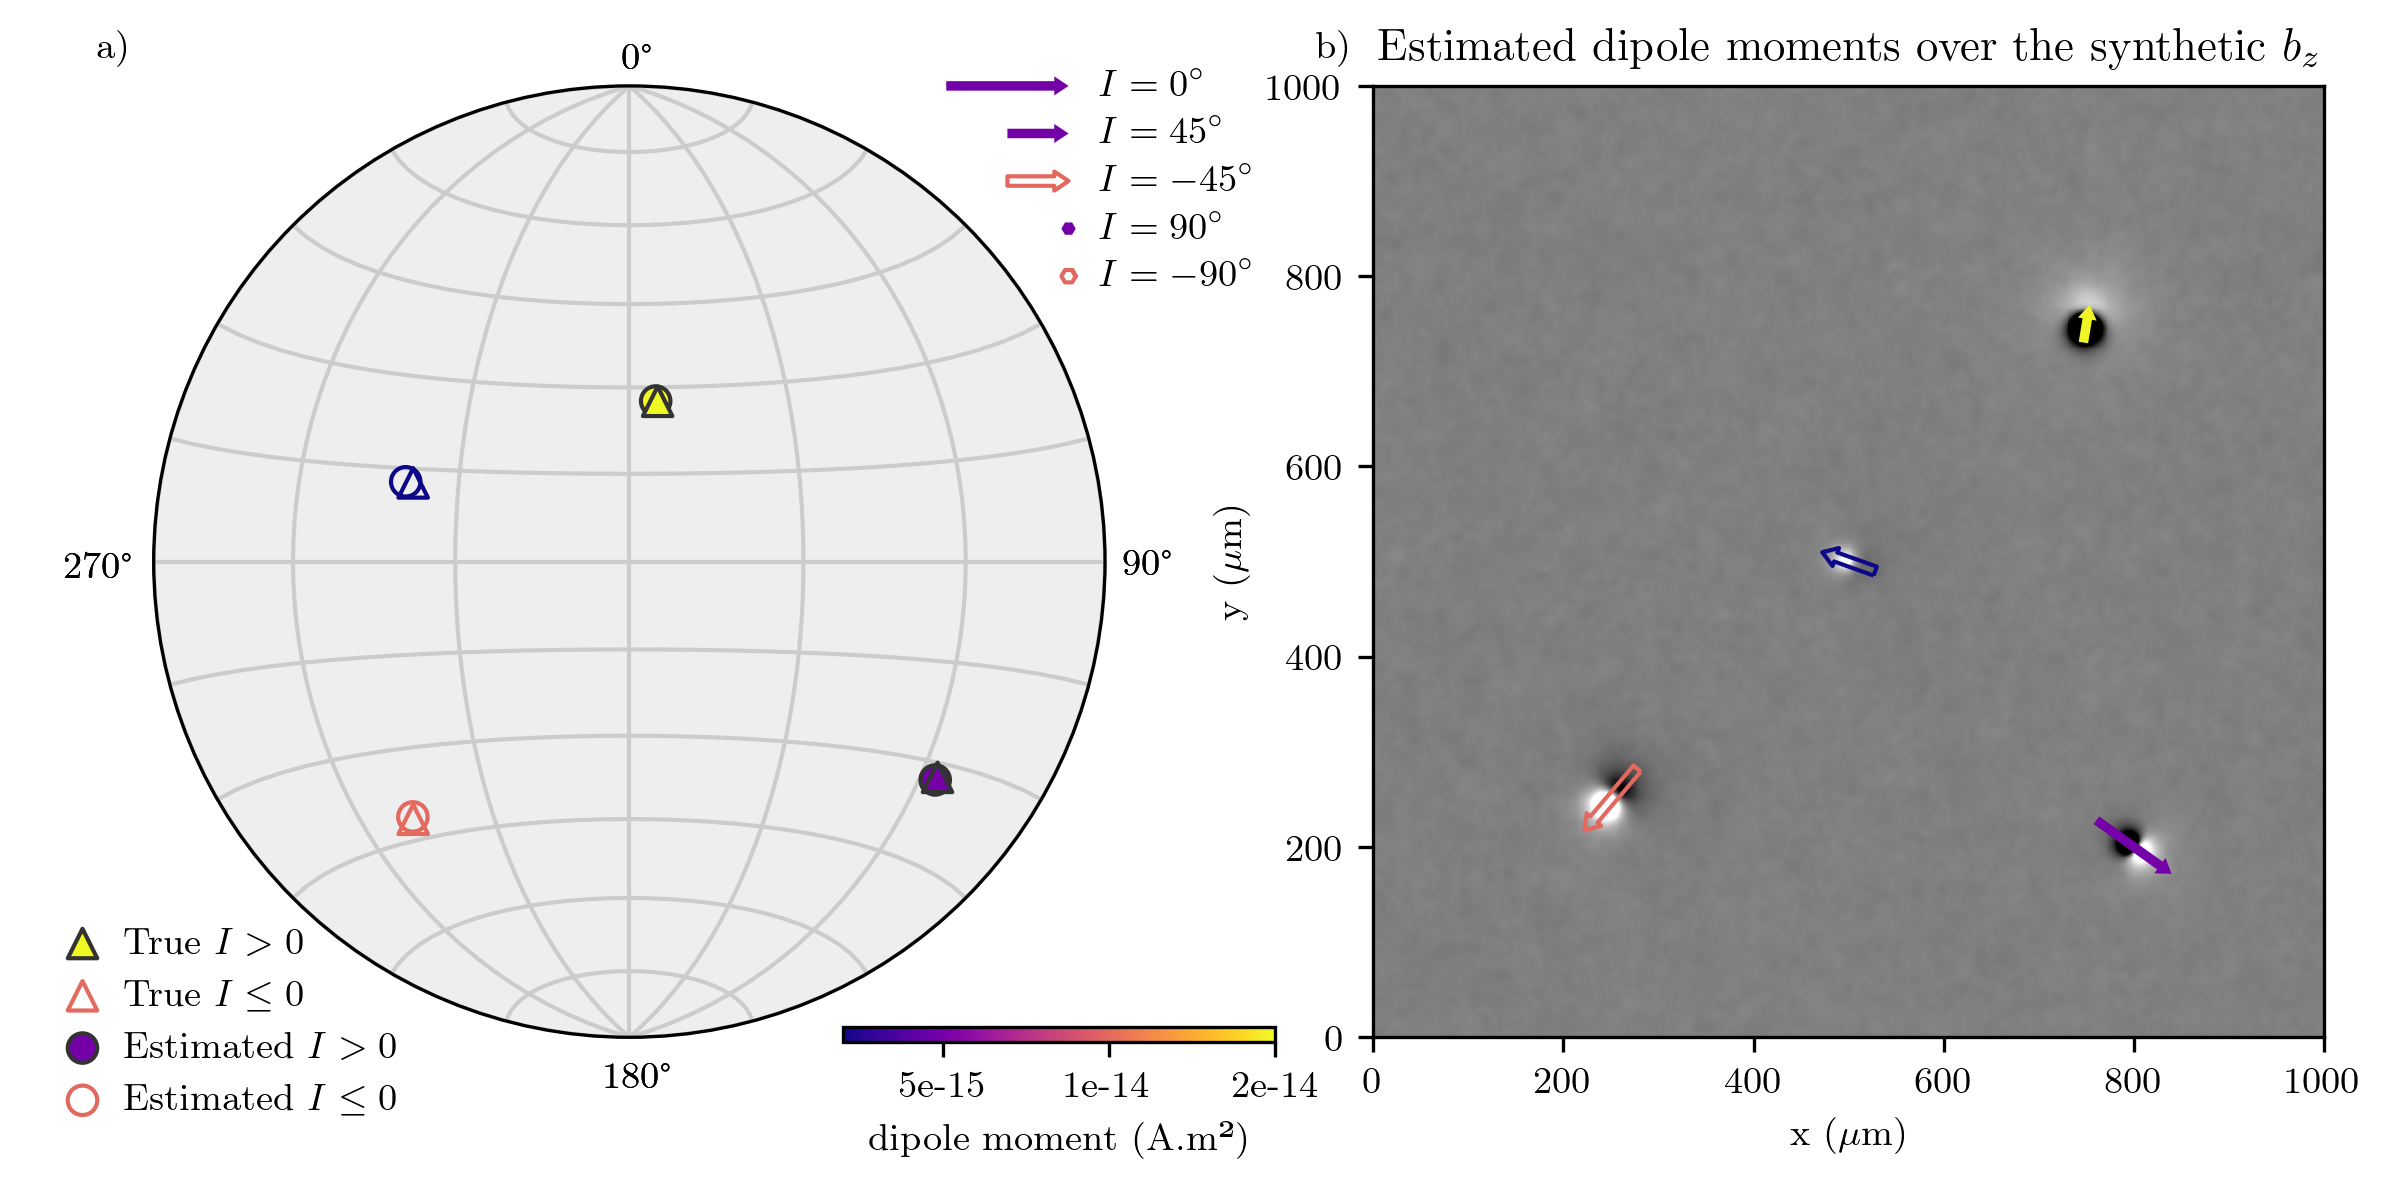
\includegraphics[width=0.75\linewidth]{figures/simple-synthetic-dipole-moment.png}
\caption{
  CAPTION NEEDED
}
\label{fig_synthetic_simple_results}
\end{figure}

The central positions of each source obtained with ED were used as an input
parameter for inverting the vertical magnetic field. The inversion produced a
least squares (or robust) approximation solution for the vector of Cartesian
magnetic moments $m_x, m_y, m_z$ and the corresponding magnetization directions
(D and I) and intensity of magnetic moment $m$. We also obtained the
uncertainty propagation of this inversion, using Equation (REFERENCE NEEDED)
and considering $\sigma = \qty{15}{\nano\tesla}$.

\begin{table}[t]
  \begin{center}
    \small
    
\begin{tabular}{ r c c c l l l } 
  \toprule
  & \multicolumn{3}{c}{Position} & \multicolumn{3}{c}{Dipole moment} \\
  & $x_c$ ($\mu$m) & $y_c$ ($\mu$m) & $z_c$ ($\mu$m) & $I$ (\textdegree) & $D$ (\textdegree) & $m$ (A.m²) \\
  \midrule
  true & 800.00 & 200.00 & -3.50 & 22.00 & 125.00 & 5.000e-15 \\
  estimated & 799.91 & 199.94 & -3.40 & 22.08 ± 0.01 & 125.52 ± 0.02 & 4.921e-15 ± 1.4e-18 \\
  true & 750.00 & 750.00 & -8.50 & 62.00 & 10.00 & 1.500e-14 \\
  estimated & 749.98 & 749.99 & -8.43 & 62.00 ± 0.01 & 9.30 ± 0.02 & 1.486e-14 ± 1.8e-18 \\
  true & 250.00 & 250.00 & -10.00 & -30.00 & -140.00 & 1.000e-14 \\
  estimated & 250.03 & 249.89 & -9.93 & -30.32 ± 0.01 & -139.70 ± 0.02 & 9.966e-15 ± 2.6e-18 \\
  true & 500.00 & 500.00 & -7.75 & -50.00 & -70.00 & 2.000e-15 \\
  estimated & 500.07 & 499.95 & -7.76 & -48.66 ± 0.05 & -70.36 ± 0.09 & 2.000e-15 ± 1.8e-18 \\
  \bottomrule
\end{tabular}

  \end{center}
  \caption{Meh}
  \label{tab_synthetic_simple_results}
\end{table}

\citet{Oliveira2015Estimation} proved that the magnetization directions (D and
I) recovered by the least squares estimator are sensitive to variations in the
horizontal coordinates of the center of the magnetic sources, but are
practically insensitive to variations in depth. Thus, they consider the Euler
deconvolution method as an adequate technique to estimate the central positions
that will be used as prior information for inversion. This occurs mainly
because, when well performed, the recovery of the horizontal coordinates of the
source central position is considerably accurate, while the vertical coordinate
can undergo greater variation even though it still provides satisfactory
results \citep{Silva20033D, Melo2013}.


\subsection{Complex simulation: Testing applicability}

This test represents a more complex scenario by simulating 100 sources randomly
distributed in the imaged area of a synthetic thin section of 2000 x 1400 $\mu
m$. The synthetic $b_z$ data were generated on a regular grid with 2 $\mu m$
spacing and 5 $\mu m$ sample-sensor distance. For greater fidelity to real
samples, the magnetic sources are modeled as spheres with different depths,
radii, and magnetizations. The depths vary between 1 and 19 $\mu m$, while the
radii range from 0.01 to 0.95 $\mu m$. The magnetizations of the sources have
declination and inclination directions sampled from a pseudo-random Gaussian
distribution with a mean of D, I = 45°, 45°, and a standard deviation of 8°.
This randomness simulates the NRM found in real ferromagnetic particles that
vary individually but average out to the inducing field direction. Finally, we
contaminated the data with high-frequency normally-distributed pseudo-random
noise with zero means and 5 nT standard deviations, as well as with
low-frequency noise in the form of additional deep sources beyond the modeling
domain. The noise-corrupted synthetic $b_z$ image is shown in
Figure~\ref{E9td9j9aBB}a.

\begin{figure}[t]
\centering
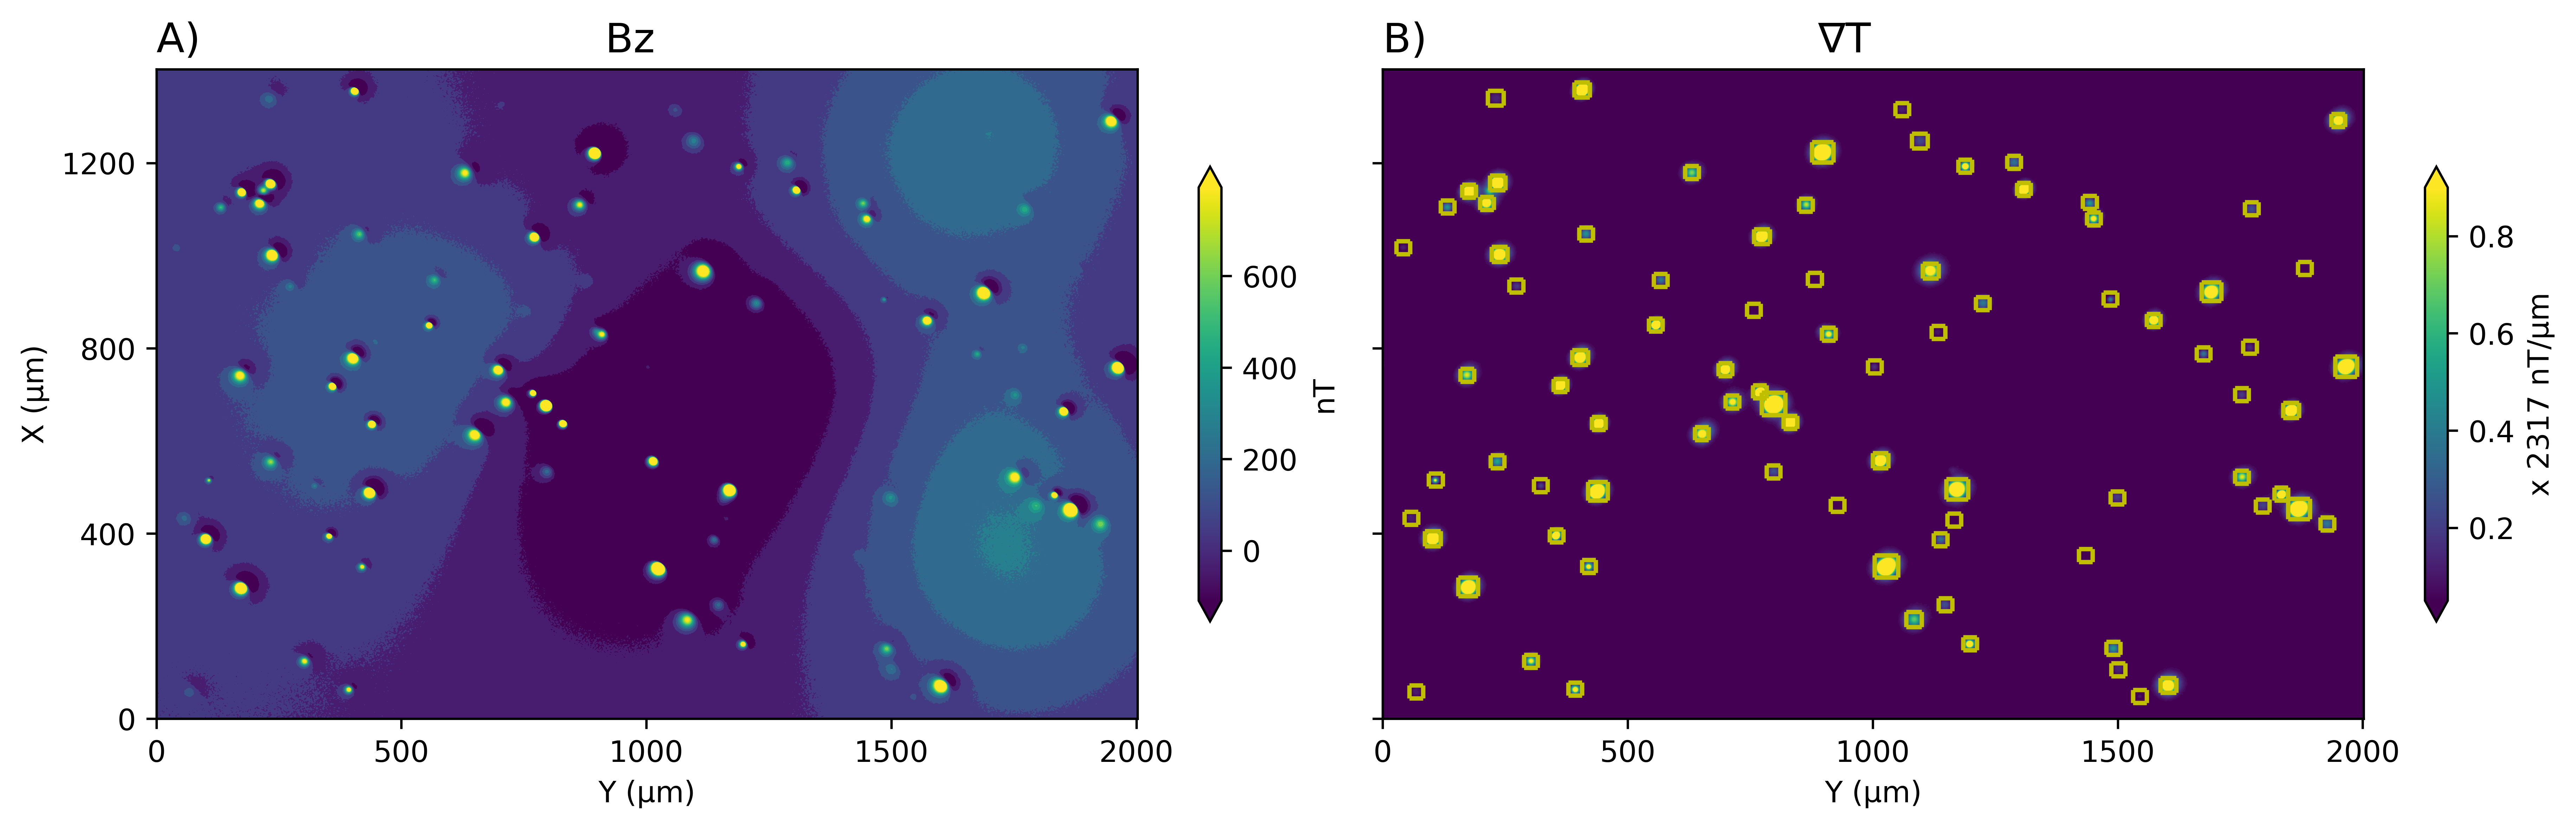
\includegraphics[width=1\linewidth]{figures/ComplexSynthetic.png}
\caption{a) Complex synthetic data contaminated with  both high and low frequencies noise. b) Individual sources' window position (yellow squares) obtained with the blob detection algorithm applied on the total gradient map.}
\label{e9td9j9abb}
\end{figure}

The result of the source detection method is shown in Figure~\ref{E9td9j9aBB}b,
where 84 particles out of the original 100 were detected. The spatiality of the
inversion results is one of the key advantages of magnetic microscopy over the
classic techniques of paleomagnetism. Therefore, we present the inversion
results spatially so that we can evaluate any patterns in their distribution.

Figure~\ref{P8gMJ9mWpS} shows the difference between the estimated dipole
moments and the true values for each of the 84 particles that were identified.
Figure~\ref{P8gMJ9mWpS}c shows the R² coefficient of determination representing
how well the dipolar model is able to fit the observed data in the given
window. The depth and radius of each particle are represented by horizontal and
vertical cross bars, respectively. The depth and radius are useful proxies for
the width and amplitude of the magnetic signal of each particle, which is
crucial to know when evaluating the inversion results.

\begin{figure}[t]
\centering
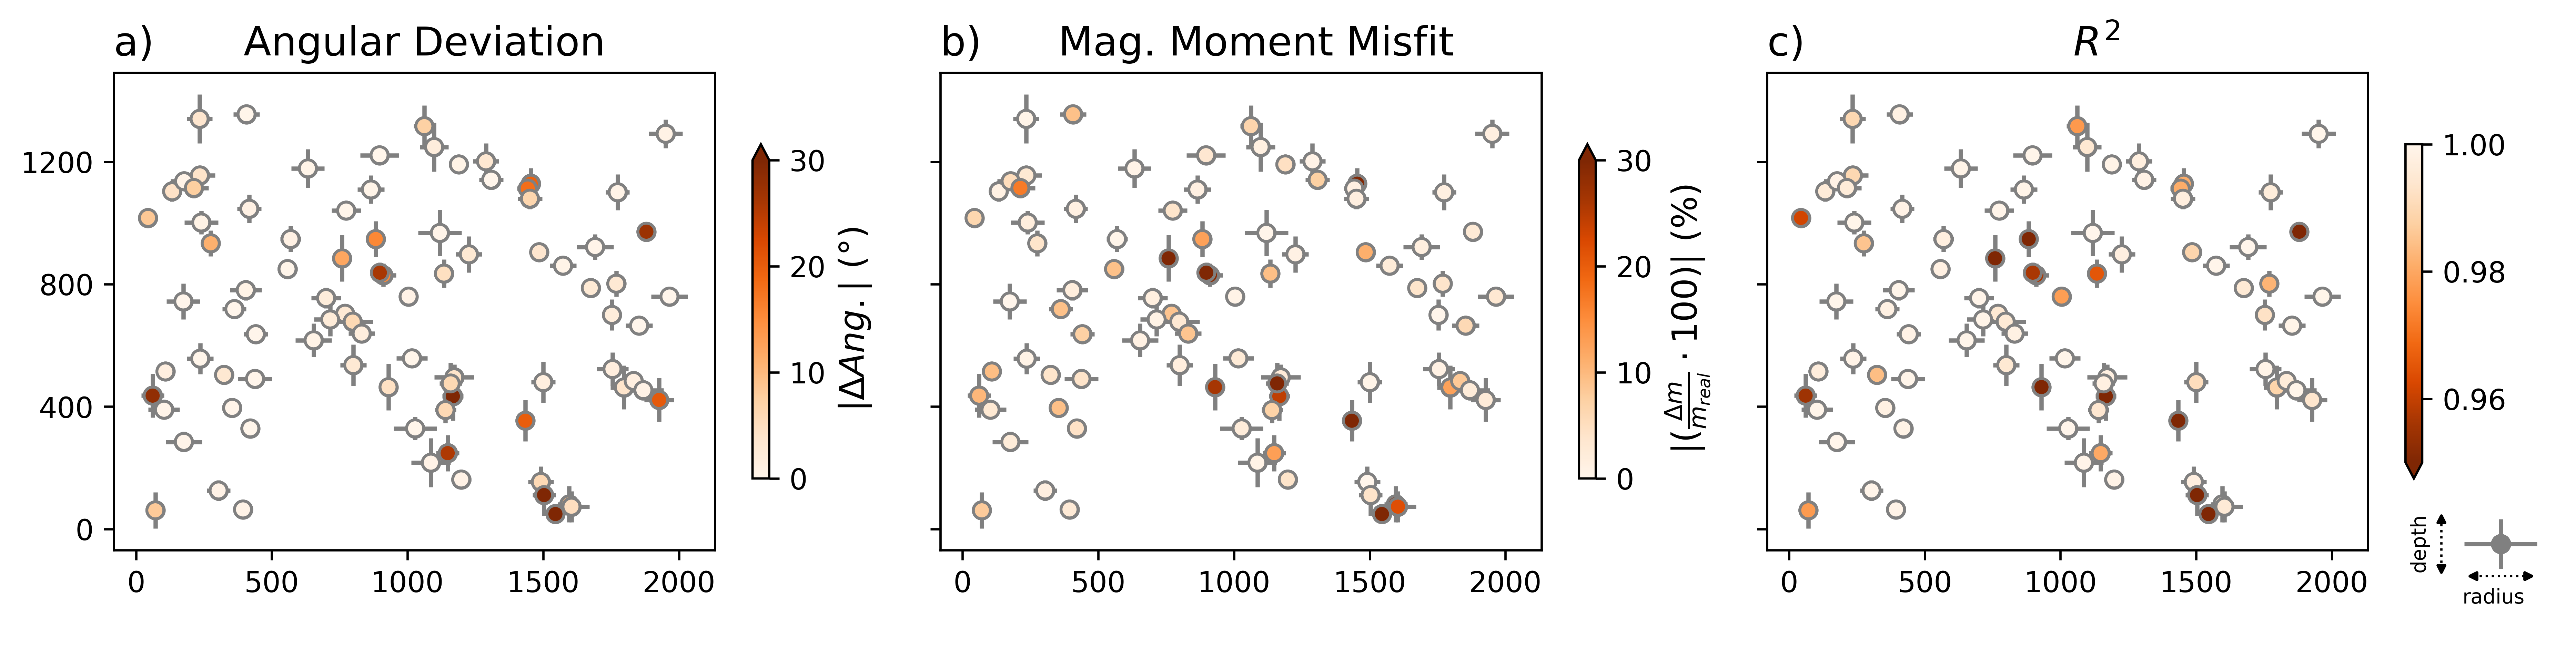
\includegraphics[width=1\linewidth]{figures/ComplexComparison.png}
\caption{
The validation of the result obtained with the inversion was calculated for
each individual particle based on the error between the real parameters modeled
and their respective recovered values, being (a) the direction and (b)
intensity of the magnetic moment, in addition to the R$^2$ score (c) obtained
by comparing the forward model and the actual data. The depth and radius of the
magnetic sources are also important factors that influence the final result,
therefore, these data are given in the form of cross plots, with the vertical
bar represented by the depth (1 - 19 $\\mu m$) and the horizontal bar by the
radius (0.01 - 0.95 $\\mu m$).
}
\label{p8gmj9mwps}
\end{figure}

The application in complex synthetic data allows observing the strengths and
limitations of the proposed methodology. Some of the strengths that can be
mentioned are: (i) the applied technique not only detects most of the modeled
sources but also (ii) most of the recovered magnetic parameters have
considerably low errors, especially in the directions, usually less than 5°
(Figure~\ref{P8gMJ9mWpS}a). (iii) The magnetic moments obtained also tend to
not deviate much from the real values (Figure~\ref{P8gMJ9mWpS}b) when
R\textsuperscript{2} scores are high (\textgreater 0.95)
(Figure~\ref{P8gMJ9mWpS}c). (iv) Shallow particles grouped in clusters are
usually well individualized during window selection, as well as (v) some
particles that produce a weak magnetic signal but isolated particles.

The main limitations observed are: (i) the blob detection fails when there are
sources too close, grouping them into the same window, thus causing an
erroneous result both for Euler deconvolution and for the magnetic parameters.
(ii) The very same occurs when there is a source under another, in this case,
the magnetic signal is the sum of both. (iii) In clusters of larger and/or
deeper particles, although the method individualizes them well, the magnetic
signal of the neighboring particles can considerably influence the result of
the inversion. Apparently, there is a direct relationship between the size and
depth with the observed errors. It is clear from the cross bars in
Figure~\ref{P8gMJ9mWpS} that deep particles and/or particles with small radii
generate worse results essentially because they will produce smaller anomalous
fields in the magnetic maps. Note nonetheless that even small particles when
close to the surface are adequately modeled by our method.

Figure~\ref{RDs2vUEqCI} shows stereoplots with the directions generated by the
model and the recovered data. The mean directions modeled are coincident with
the model and the distribution is coincident within the 95\% confidence cone.
When filtered to include only data with R\textsuperscript{2} \textgreater 0.95
the obtained directions are closer to the model average and less sparse.

\begin{figure}[!htbp]
\centering
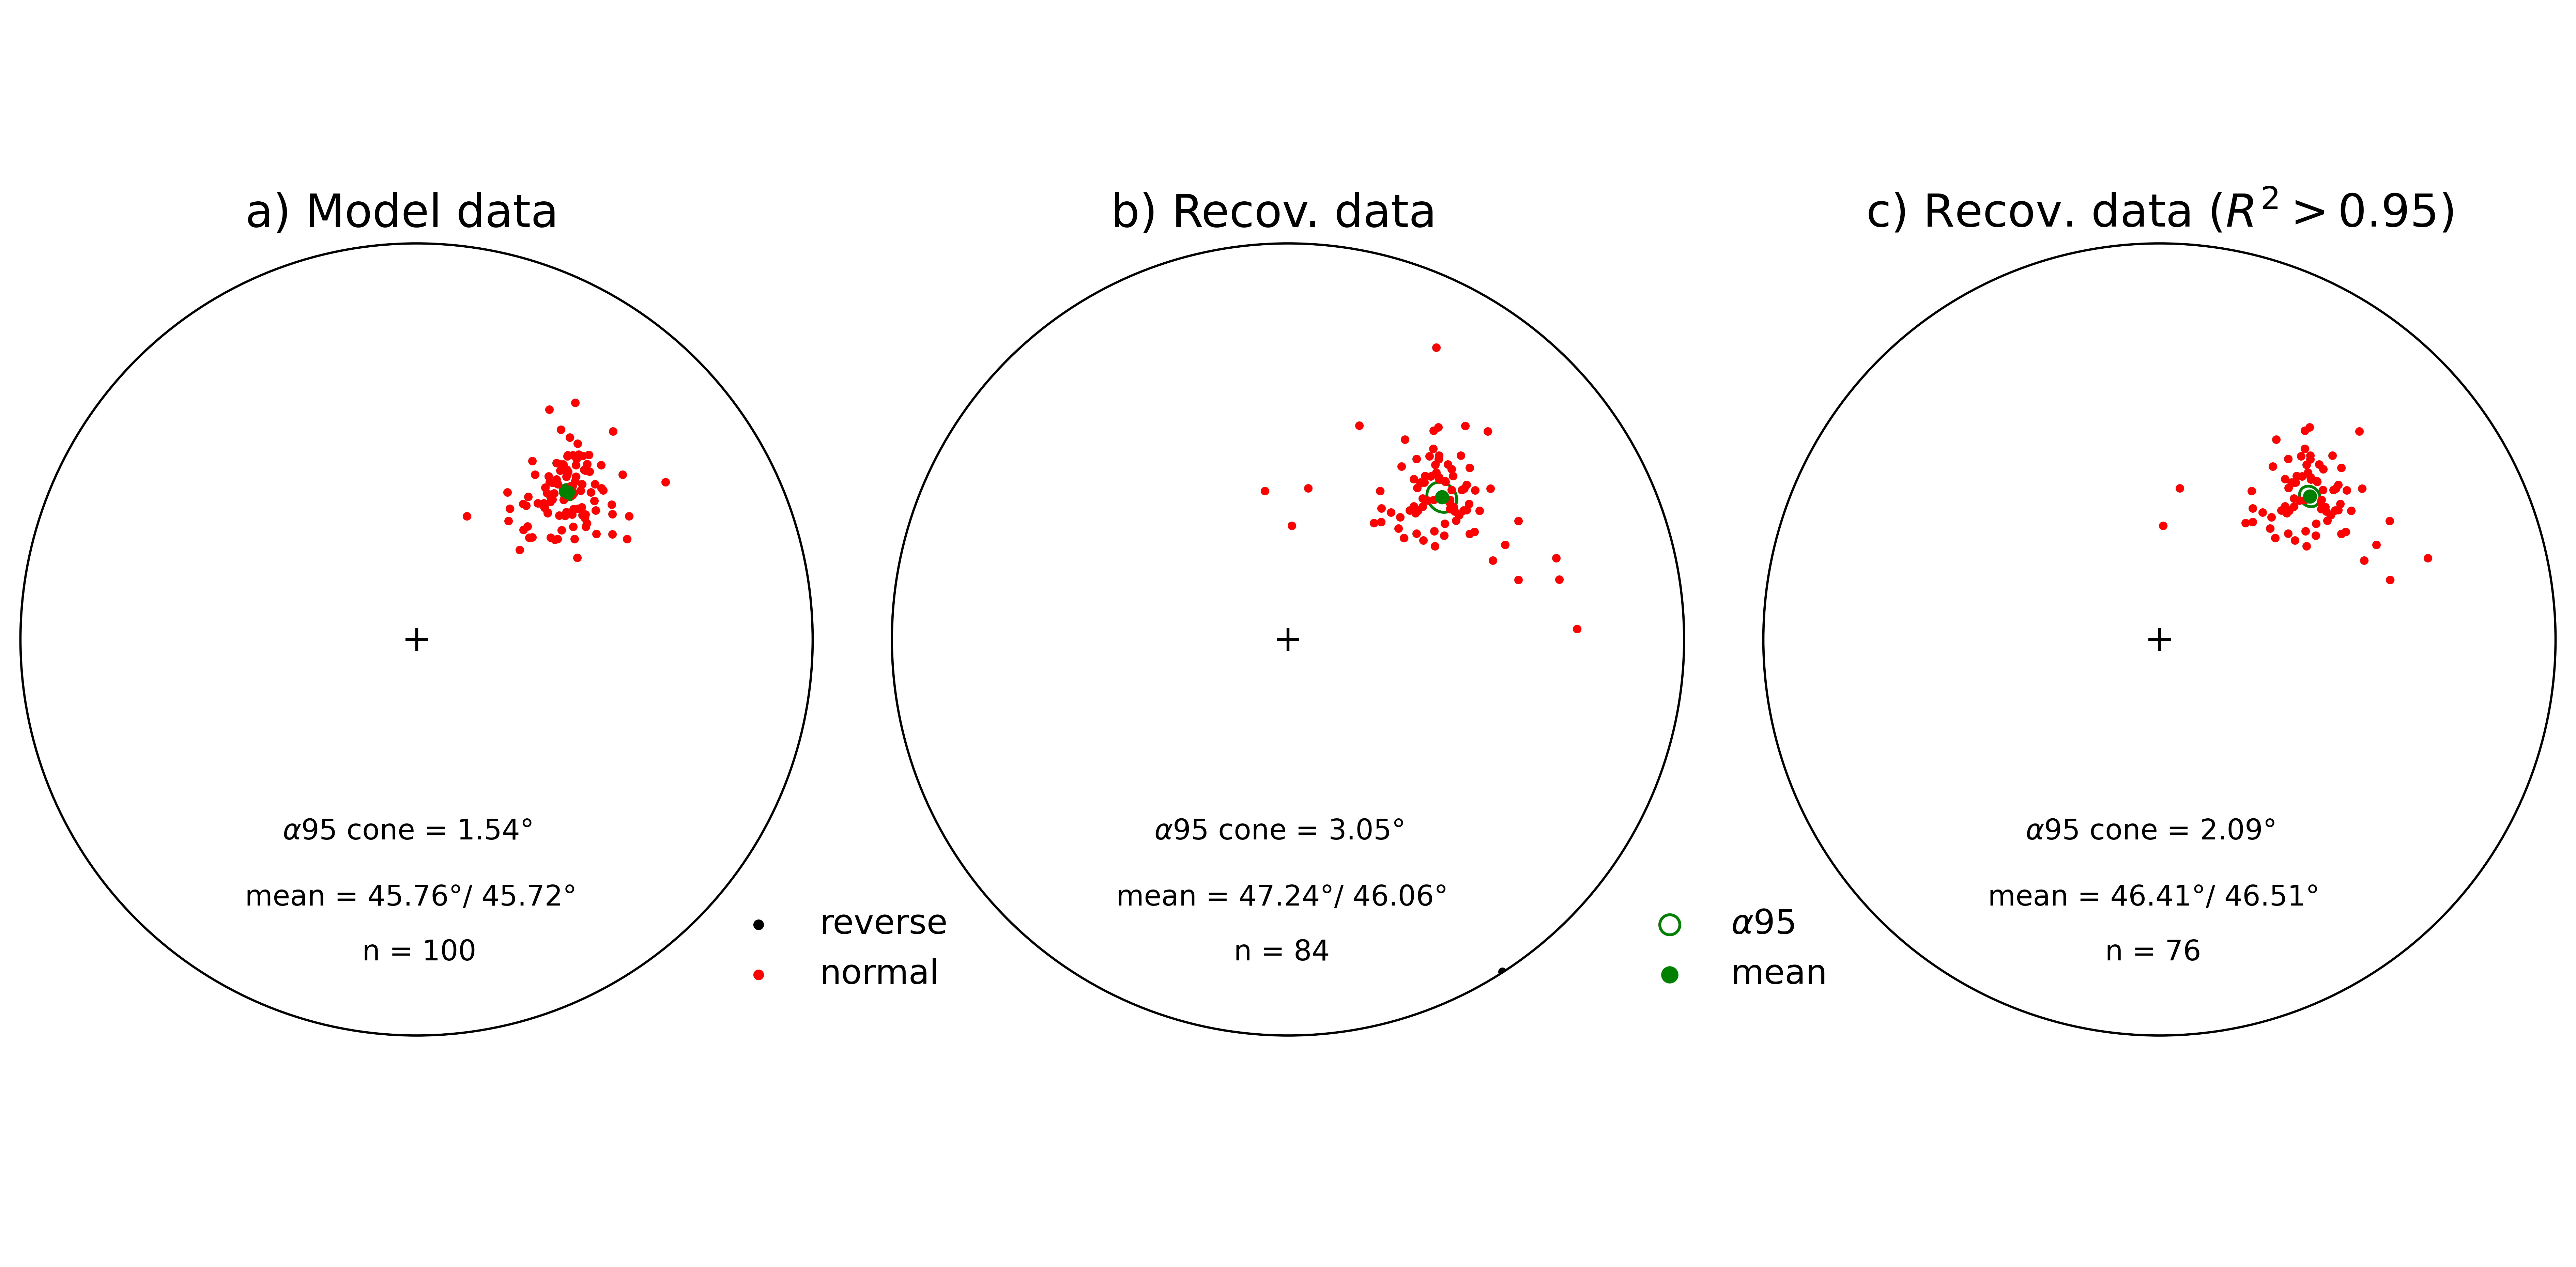
\includegraphics[width=1\linewidth]{figures/ComplexStereo.png}
\caption{
a) Simulation of a thin section of rock with particles uniformly magnetized in
the average direction of the induced field
45{\textbackslash}textdegree/45{\textbackslash}textdegree. b) The recovered
data, without any type of filtering, are sparse, but statistically generate the
same average direction. c) It is still possible to filter only the directions
of the magnetic sources with the best fitting determined by the coefficient of
determination ($R^ 2 \\geq 0.95$) to ensure better grouping of the directions
around the mean value.
}
\label{rds2vueqci}
\end{figure}



%%%%%%%%%%%%%%%%%%%%%%%%%%%%%%%%%%%%%%%%%%%%%%%%%%%%%%%%%%%%%%%%%%%%%%%%%%%%%%%
\section{Application to real data}

To test whether the proposed method would be able to determine the
magnetization directions and the magnetic moment of particles in natural
samples, we selected a previously studied carbonate stalagmite sample from the
Wintimdouine cave in the Agadir region (Morocco) \citep{Ait2019Hydro}. This
speleothem contains both magnetite and hematite as the main carriers of
magnetic remanence, as attested by thermomagnetic curves with temperature
decays at {\textasciitilde}580 °C and {\textasciitilde}680 °C, and bimodal
curves of isothermal remanent magnetization (IRM) acquisition (Carmo et al.,
2019).

In order to provide two distinct directions associated with the different
magnetic mineral types in this sample, we applied two IRM pulse fields of 2.7 T
and 0.3 T, respectively toward the +X and -X directions. In this way, the high
coercivity grains (hematite) would point towards +X and the low coercivity ones
(magnetite) would align in the -X direction.

After remanence acquisition, we performed a magnetic map with the Quantum
Diamond Microscope (QDM) at Harvard University over a sample section of
approximately 1410 $\mu$m x 2256 $\mu$m (Figure~\ref{W1GfysVYnX}a) with a grid
spacing of 2.35 $\mu$m and a sensor-sample distance of 5 $\mu$m, totaling
576x10\textsuperscript{3} data points. The QDM is housed in a shielded room, in
order to avoid the influence of the Earth's magnetic field \citep{Fu2020,
Glenn2017}. After applying the magnetic anomaly detection algorithm, it was
possible to determine the windows for 85 potential sources
(Figure~\ref{W1GfysVYnX}b).

\begin{figure}[tb]
\centering
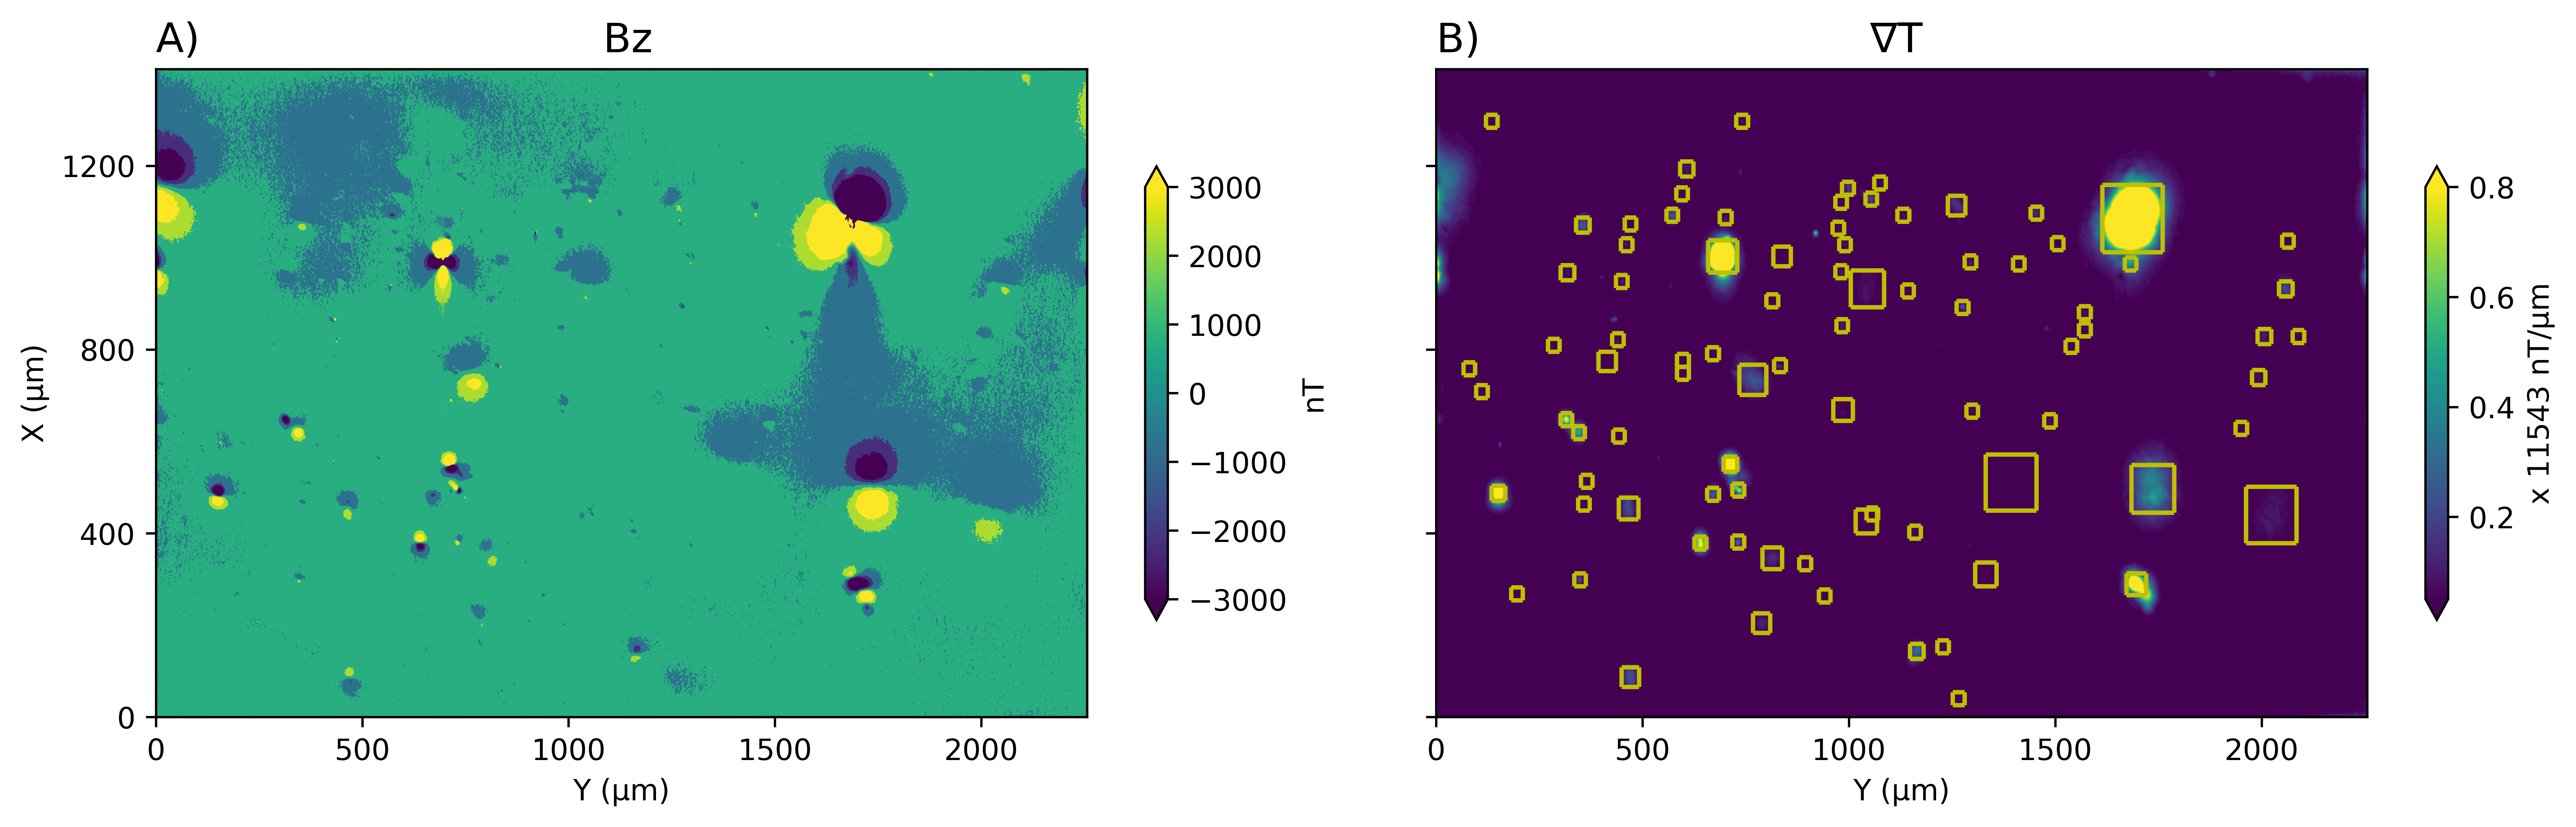
\includegraphics[width=1\linewidth]{figures/RealData.png}
\caption{
a) Real sample data. b) Individual sources' window position (yellow squares)
obtained with the blob detection algorithm applied on the total gradient map.
}
\label{w1gfysvynx}
\end{figure}

After applying the ED algorithm, we performed the inversion of the magnetic
moment for each of the 85 windows selected previously. In order to reduce
considerably the computation time, the inversions were done within each data
window, instead of solving all sources parameters at the same time. We obtained
the magnetic moment (not shown) and the direction for all 85 magnetic grains
(Figure~\ref{NKOAMThaWA}a). Then, we calculated the residuals of the inversions
in each window and subsequently the coefficient of determination
R\textsuperscript{2}, which was used as a filter for the best directions
obtained. We used a cut-off limit of the coefficient of determination at 0.7
(Figure~\ref{NKOAMThaWA}b) EXPLICAR PORQUE USOU 0.7 AQUI E 0.95 NOS CASOS
SINTÉTICOS. This filtering technique removed unreliable responses showing more
clearly the expected directional clusters of hematite and magnetite crystals.
NÃO SABEMOS SE OS PONTOS RETIRADOS SÃO `UNRELIABLE RESPONSES'\dots ALÉM DISSO,
O FILTRO ELIMINA QUASE 50\% DAS FONTES IDENTIFICADAS, O QUE PODE SER UM
PROBLEMA SE TIVERMOS QUE APLICAR EM OUTROS CASOS REAIS. USAR O TESTE DE
NÃO-DIPOLARIDADE? TALVEZ SEJA MAIS INTERESSANTE, DADA A DISCUSSÃO QUE SEGUE.

\begin{figure}[tb]
\centering
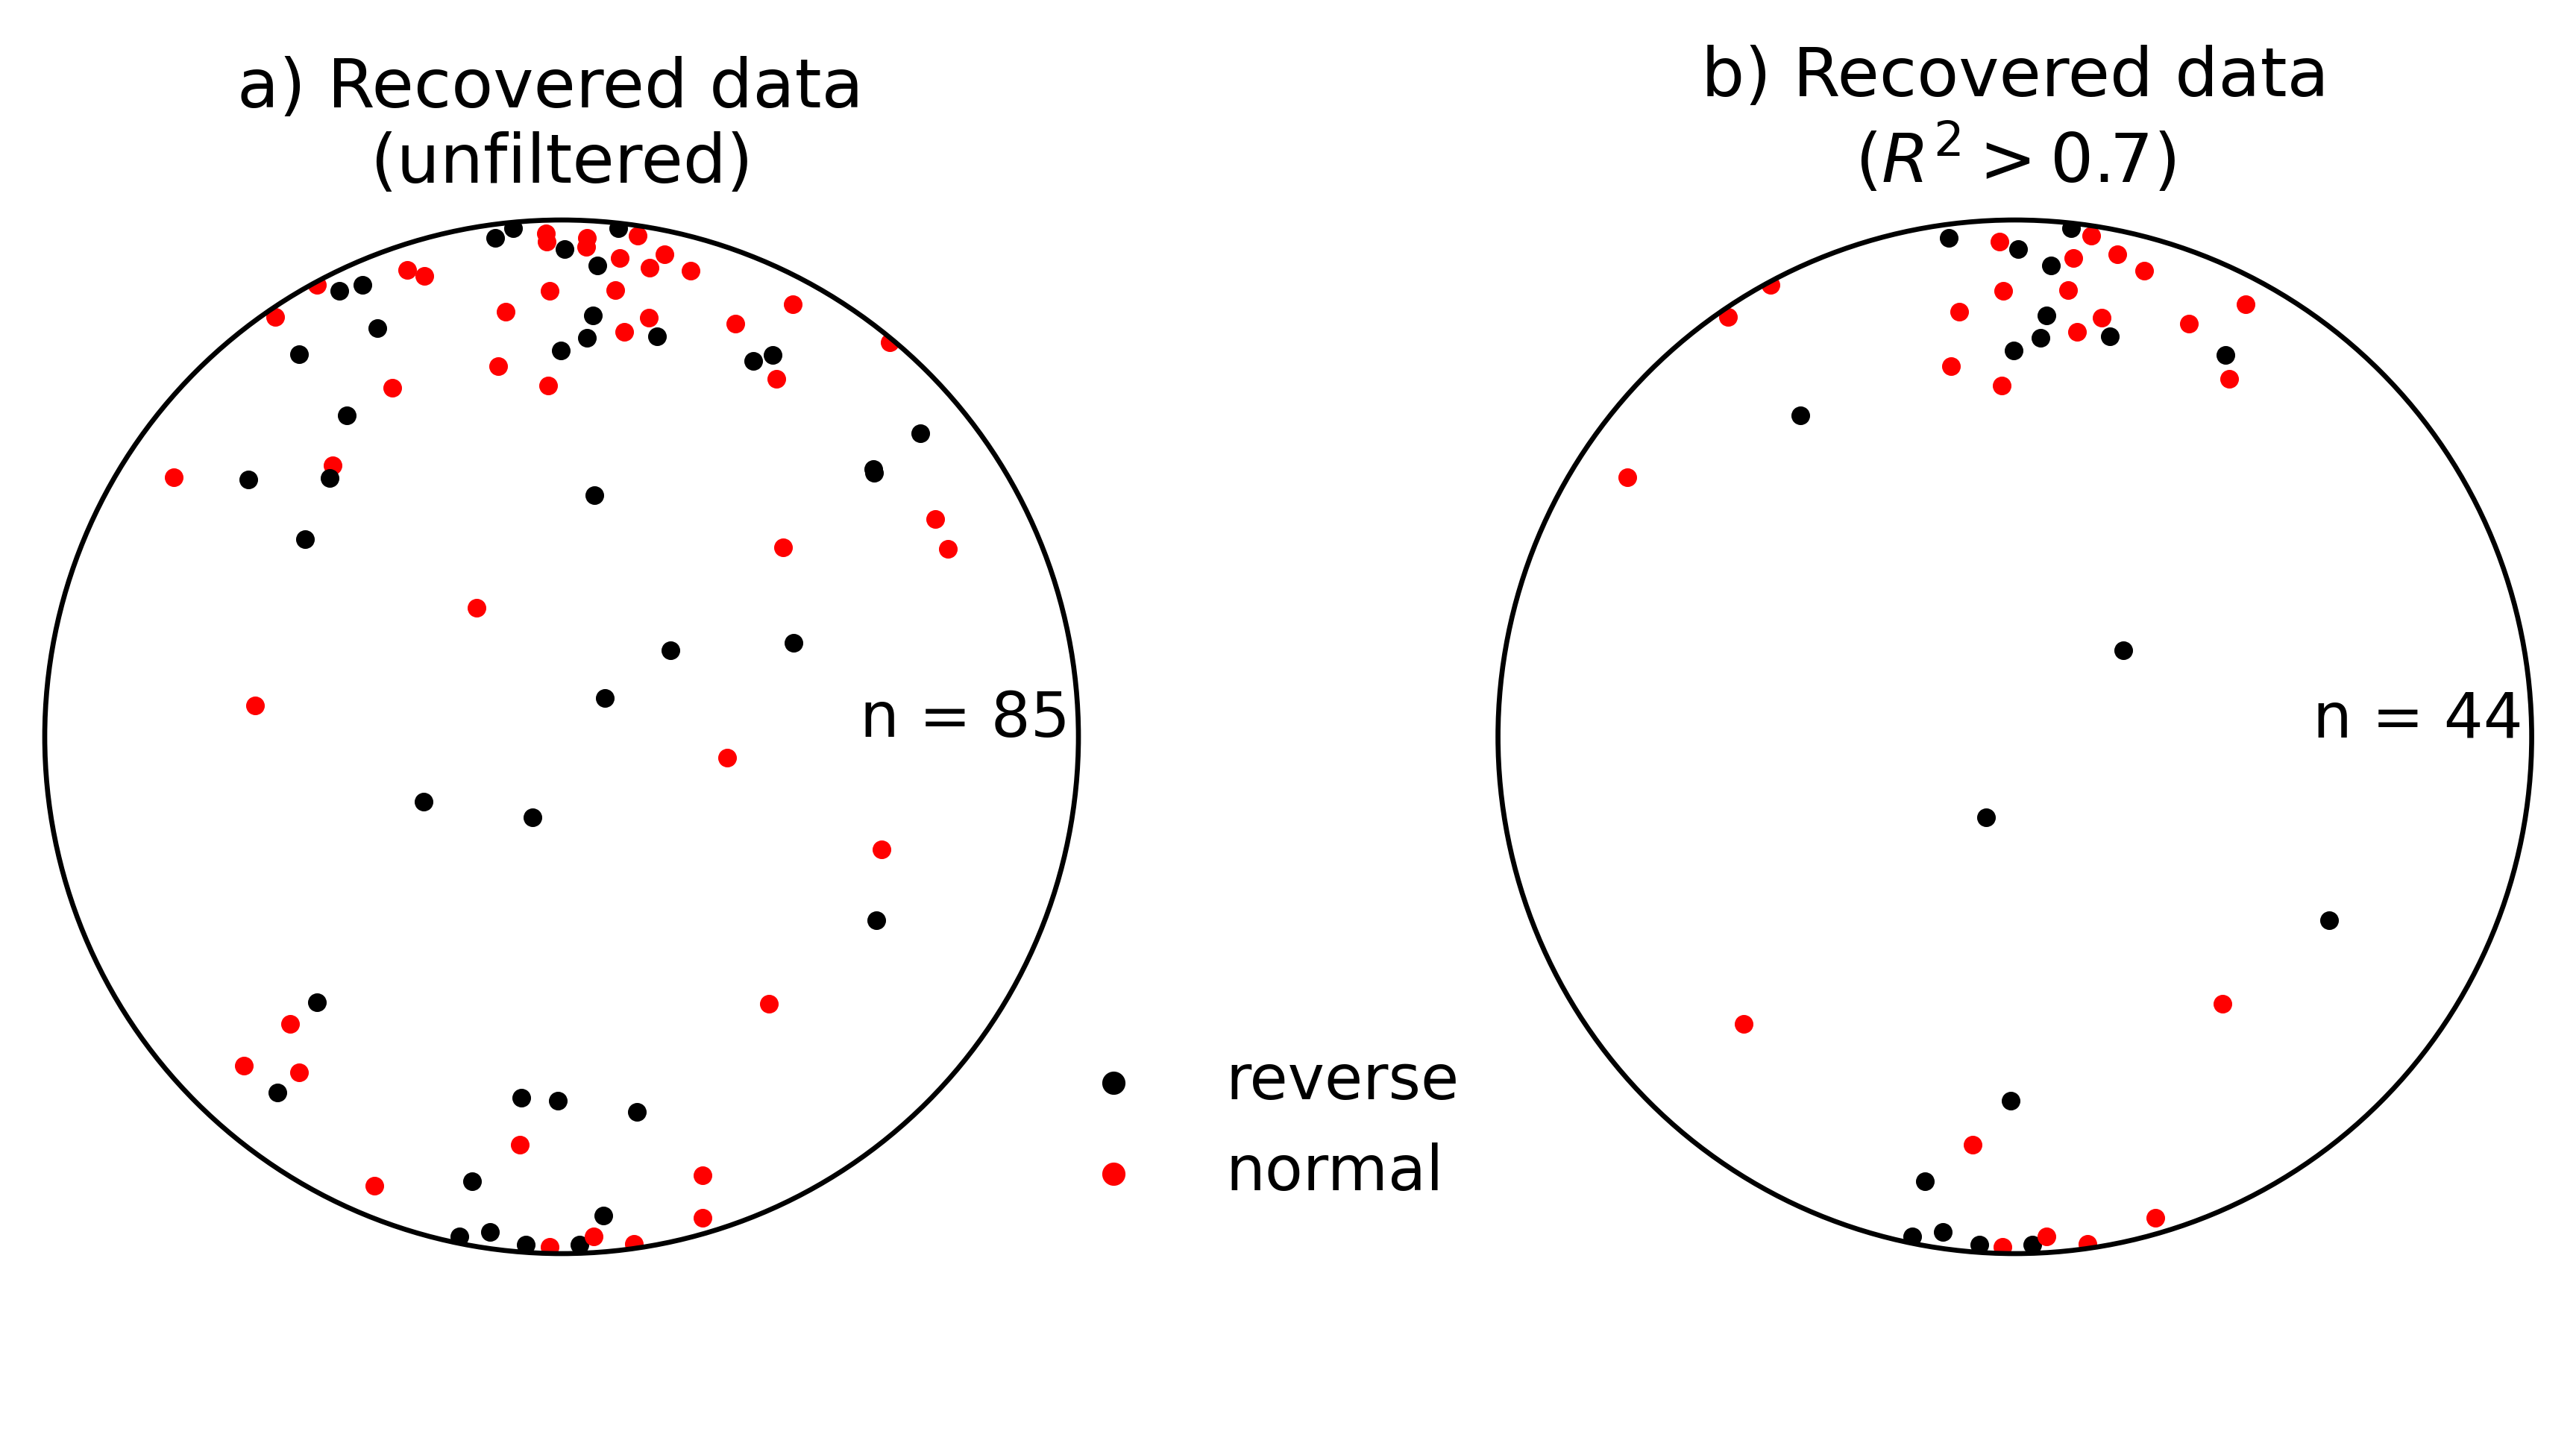
\includegraphics[width=1\linewidth]{figures/RealDataStereo.png}
\caption{
a) The recovered data, without any type of filtering. b) Recovered data
filtered by the coefficient of determination ($R^ 2 \\geq 0.7$), which shows
two clusters of direction located on each pole of the stereogram.
}
\label{nkoamthawa}
\end{figure}

NESSA PARTE SERIA INTERESSANTE INCLUIR MAPAS COMO OS DA FIGURA 4B E 4C, COM A
ESPACIALIDADE DOS AJUSTES E DISCUTIR DA SEGUINTE FORMA:

\begin{enumerate}
\item RESULTADOS EM FUNÇÃO DA QUALIDADE DO AJUSTE
\item RESULTADOS EM FUNÇÃO DA DIPOLARIDADE DAS FONTES
\item CONTEXTUALIZAR O SEU MÉTODO EM RELAÇÃO A OUTROS. COMO OS OUTROS ESTIMAM
  OS MISFITS? QUE FILTROS USAM? QUAL A DIFERENÇA COM SUA ABORDAGEM? POR
  ENQUANTO SOMENTE O TRABALHO DE CORTEZ ESTÁ COMENTADO -> COMPARAR COM
  OS OUTROS MÉTODOS DE INVERSÃO (Fu, de Groot, Egli2000, Lima2007)
\end{enumerate}

The application of the proposed algorithm to natural samples gives some
indications of its ability to circumvent the prominent problems described by
\citep{CortesOrtuno2022} [QUAIS PROBLEMAS FORAM LISTADOS POR CORTÉS-ORTUÑO?],
namely: (i)\dots, (ii)\dots, (iii)\dots

the same authors showed that particles in the single vortex PSD state present
more accurate inversion results when considering the non-dipole components for
small sample-sensor distances (\textless 1 $\mu$m), but for larger sensor
distances the dipole as approximations are remarkably accurate, as the
higher-order moments decay rapidly with distance and therefore have less
influence on the particle's magnetic signal. Thus, our approach can be
considered reasonable for working with particle signals in SD (already a
dipole) and PSD states. The latter happens due to the QDM sensor height being
usually greater than 5 $\\mu m$, considering a particle on the immediate
surface of the sample the higher-order moments are already quite attenuated.\}

Despite the excellent signal/noise ratio that the SMM provided with the
proximity of the sensor to the sample, it is worth mentioning that the
measurement noise can still overshadow the responses of very weak/small, or
deep particles, generating unreliable inversion results. Therefore, it is
necessary to keep a check to determine if the inversion reached a satisfactory
result, such as the coefficient of determination that we used or the
signal-to-noise ratio presented by \citep{CortesOrtuno2022}.


%%%%%%%%%%%%%%%%%%%%%%%%%%%%%%%%%%%%%%%%%%%%%%%%%%%%%%%%%%%%%%%%%%%%%%%%%%%%%%%
\section{Conclusion}

We developed an efficient semi-automated method to determine the direction of
magnetization of dipolar sources on a microscale, as well as the recovery of
their magnetic moment. Being ideal for a reinterpretation for the application
of methods of paleomagnetic studies using thin sections of rock samples. This
would be an attempt to improve the quality of results obtained by isolating the
responses of more reliable recorders of the Earth's geomagnetic field.

We also present a new, faster, and cleaner way to solve the Euler equation in
determining the positioning of magnetic anomaly sources using a pre-selection
of magnetic anomaly source windows based on the Laplacian of the Gaussian
applied to total gradient anomaly maps. In this way, reducing the numerous
solutions to just one data window per source. After estimating the structural
index ($n = 3$) by approximating the sources generating the magnetic anomaly to
spheres/points, the Euler deconvolution is performed and the central position
of each source is determined.

The recovery of direction and magnetization we only need to assume that the
sources have their central positions known (so we apply Euler deconvolution)
and that their magnetizations are uniform. This last premise aligns with the
theory of magnetically stable particles SD (and the PSD ones at a reasonable
sensor height), which is the basis of classical paleomagnetism. Also, there is
no need for any kind of prior knowledge other than the observed magnetic
anomaly, and the structural index of the sources. Therefore, this method can be
quickly replicated in a dataset of thin sections of rocks to obtain the
distributions of magnetic directions of each source identified in the sample.

The test using a simple synthetic sample shows the great capability of the
method by retrieving not only the precise center positions, but also retrieving
the magnetization directions and intensity even under the considerable effect
of high-frequency noise (15 nT). While the complex synthetic sample data allows
observing the applicability of the method developed in real samples that are
more complex with varied magnetization directions and intensity, in addition to
also taking into account the high and low-frequency noise and sources with
variable sizes and depths.

The real sample data positively answered the question of the algorithm's
ability to deal with rocks thin-sections. But also, showed the acceptable
capacity (within the adequate R$^2$ threshold) of retrieving different
magnetization directions recorded by magnetic minerals with different
coercivities and magnetic signal disparities even greater than predicted in the
complex synthetic test.



%%%%%%%%%%%%%%%%%%%%%%%%%%%%%%%%%%%%%%%%%%%%%%%%%%%%%%%%%%%%%%%%%%%%%%%%%%%%%%%
\section{Data and code availability}

The Python source code used to produce all results and figures presented here
is available at \url{https://github.com/\GitHubRepository} and
\url{https://doi.org/\ArchiveRepository} under the MIT open-source license.

The image rescaling and blob detection though the Laplacian of Gaussian method
were performed with the scikit-image library \citep{VanderWalt2014}. CITE OTHER
SOFTWARE TOOLS USED. Matplotlib for figures, numpy and scipy for almost
everything. Verde for the regional residual separation and other things.

The QDM image data is available at CITE A DATAVERSE/FIGSHARE ARCHIVE under the
CC-XX license.



%%%%%%%%%%%%%%%%%%%%%%%%%%%%%%%%%%%%%%%%%%%%%%%%%%%%%%%%%%%%%%%%%%%%%%%%%%%%%%%
\section{Acknowledgements}

We are indebted to the developers and maintainers of the open-source software
without which this work would not have been possible.


\bibliographystyle{apalike-doi}
\bibliography{references}

\end{document}
